% TODO:
% - integrate description of splitters
% - possibly show screenshots from all videos?

\startchapter{Translating Stream Programs into the Compressed Domain}
\label{chap:compression}

%YouTube manages about 45 terabytes of video data~\cite{wsj-youtube},
%with 65,000 videos uploaded daily~\cite{youtube}.  Microsoft
%TerraServer holds upwards of 22 terabytes of image data, serving 69
%gigabytes per day~\cite{terraserver}.

This chapter presents a new domain-specific optimization for stream
programs: translation to the compressed domain.  This transformation
allows programs to operate directly on compressed data, accelerating
common video editing operations by a median of 15x.  Unlike the
optimization of linear nodes in StreamIt, this represents a
domain-specific optimization that was previously unknown (it was not
performed even by experts).  We define the transformation in general
terms and also evaluates it experimentally in the context of StreamIt.

\section{Introduction}

Stream programs often operate on huge volumes of data.  For example,
each frame of a digital film requires approximately 2 megabytes,
implying that a fully-edited 90-minute video demands about 300
gigabytes of data for the imagery alone~\cite{ibm-video}.  Industrial
Light and Magic reports that, in 2003, their processing pipeline
output 13.7 million frames and their internal network processed 9
petabytes of data~\cite{ilm-interview}.  The U.S. Geological Survey
had archived over 13 million frames of photographic data by the end of
2004, and estimates that 5 years is needed to digitize 8.6 million
additional images~\cite{usgs}.  In all of these situations, the data
is highly compressed to reduce storage costs.  At the same time,
extensive post-processing is often required for adding captions,
watermarking, resizing, compositing, adjusting colors, converting
formats, and so on.  As such processing logically operates on the
uncompressed format, the usual practice is to decompress and
re-compress the data whenever it needs to be modified.

In order to accelerate the process of editing compressed data,
researchers have identified specific transformations that can be
mapped into the compressed domain---that is, they can operate directly
on the compressed data format rather than on the uncompressed
format~\cite{chang95survey,mandal95survey,smith95survey,wee02survey}.
In addition to avoiding the cost of the decompression and
re-compression, such techniques greatly reduce the total volume of
data processed, thereby offering large savings in both execution time
and memory footprint.  However, existing techniques for operating
directly on compressed data are largely limited to lossy compression
formats such as
JPEG~\cite{dugad01,feng03,mukherjee02,shen96b,shen96,shen98,smith96b}
and MPEG~\cite{smith98,dorai00,nang00,vasudev98,wee02survey}.  While
these formats are used pervasively in the distribution of image and
video content, they are rarely used during the production of such
content.  Instead, professional artists and filmmakers rely on
lossless compression formats (BMP, PNG, Apple Animation) to avoid
accumulating artifacts during the editing process.  Given the
computational intensity of professional video editing, there is a
large demand for new techniques that could accelerate operations on
lossless formats.

In this chapter, we present a technique for translating stream
programs to operate directly on losslessly-compressed data.  We
consider compression formats that are based on LZ77, a compression
algorithm that is utilized by ZIP and fully encapsulates common
formats such as Apple Animation, Microsoft RLE, and Targa.  The
transformation is most efficient when each element of a stream is
transformed in a uniform way (e.g., adjusting the brightness of each
pixel).  However, it also applies to cases in which multiple items are
processed at once (e.g., averaging pixels) or in which multiple
streams are split or combined (e.g., compositing frames).

%% However, existing techniques for operating directly on compressed data
%% have two limitations.  First, they focus on lossy compression formats
%% (e.g., JPEG, MPEG) rather than lossless compression formats; lossless
%% compression is the new standard for professional video editing and
%% movie production.  Second, they rely on specialized and ad-hoc
%% techniques for translating individual operations into the compressed
%% domain.  For example, for DCT-based spatial compression formats (JPEG,
%% Motion-JPEG), researchers have developed separate algorithms for
%% resizing~\cite{dugad01,mukherjee02}, edge
%% detection~\cite{shen96b,shen96}, image segmentation~\cite{feng03},
%% shearing and rotating inner blocks~\cite{shen98}, and arbitrary linear
%% combinations of pixels~\cite{smith96b}.  Techniques extending to
%% DCT-based temporal compression (MPEG) include
%% captioning~\cite{nang00}, reversal~\cite{vasudev98}, distortion
%% detection~\cite{dorai00}, transcoding~\cite{smith98}, and
%% others~\cite{wee02survey}.  For run-length encoded images, algorithms
%% have been devised for efficient transpose and
%% rotation~\cite{misra99,shoji95}.  A compressed audio format has been
%% invented that allows direct modification of pitch and playback
%% speed~\cite{levine98}.  While these techniques are powerful, they
%% remain inaccessible to most application programmers because they
%% demand intricate manipulation of the underlying compression format.
%% It is difficult for non-experts to compose existing compressed-domain
%% operations into a complete program, let alone translate a new and
%% unique operation into the compressed domain.

%% This paper presents a technique for automatically mapping complete
%% user-defined programs into the compressed domain.  The technique
%% applies to stream programs: a restricted but practical class of
%% applications that perform regular processing over long data sequences.
%% Stream programming captures the essential functionality needed by
%% image, video, and signal processing applications while exposing the
%% flow of data to the compiler.  Our formulation is based on LZ77, a
%% lossless compression algorithm utilized by ZIP, and naturally applies
%% to formats such as Apple Animation, Microsoft RLE, and Targa (which
%% are special cases of LZ77).  
%% %Lossless compression is widely used in
%% %computer animation and digital video editing in order to avoid
%% %accumulating compression artifacts.  
%% By providing an automatic mapping into the compressed domain, our
%% technique enables a large class of transformations to be customized by
%% the user and directly applied to the compressed data.

The key idea behind our technique can be understood in simple terms.
In LZ77, compression is achieved by indicating that a given part of
the data stream is a repeat of a previous part of the stream.  If a
program is transforming each element of the stream in the same way,
then any repetitions in the input will necessarily be present in the
output as well.  Thus, while new data sequences need to be processed
as usual, any repeats of those sequences do not need to be transformed
again.  Rather, {\it the repetitions in the input stream can be
  directly copied to the output stream}, thereby referencing the
previously-computed values.  This preserves the compression in the
stream while avoiding the cost of decompression, re-compression, and
computing on the uncompressed data.  

%In this paper, we extend this simple idea to a broad class of
%programs: those which input and output multiple data items at a time,
%and those which split, combine, and reorder the data in the stream.

In this work, we extend this simple idea to encompass a broad class of
programs that can be expressed in StreamIt.  We have implemented a
subset of our general technique in the StreamIt compiler.  The end
result is a fully-automatic system in which the user writes programs
that operate on uncompressed data, and our compiler emits an optimized
program that operates directly on compressed data.  Our compiler
generates plugins for two popular video editing tools (MEncoder and
Blender), allowing the optimized transformations to be used as part of
a standard video editing process.

Using a suite of 12 videos (screencasts, animations, and stock
footage) in Apple Animation format, our transformation offers a
speedup roughly proportional to the compression factor.  For
transformations that adjust a single video (brightness, contrast,
color inversion), speedups range from 2.5x to 471x, with a median of
17x.  For transformations that combine two videos (overlays and
mattes), speedups range from 1.1x to 32x, with a median of 6.6x.  We
believe this is the first demonstration of compressed-domain
techniques for losslessly compressed video content.

In the general case, compressed processing techniques may need to
partially decompress the input data to support the behavior of certain
programs.  Even if no decompression is performed, the output may
benefit from an additional re-compression step if new redundancy is
introduced during the processing (for example, increasing image
brightness can whiteout parts of the image).  This effect turns out to
be minor in the case of our experiments.  For pixel transformations,
output sizes are within 0.1\% of input sizes and often (more than half
the time) are within 5\% of a full re-compression.  For video
compositing, output files maintain a sizable compression ratio of 8.8x
(median) while full re-compression results in a ratio of 13x (median).

In the remainder of the chapter, we give an overview of LZ77
compression before describing our technique and its compatibility with
popular file formats.  We then present an experimental evaluation
before closing with related work and a chapter summary.

% HELPER FOR REPEATS:
\newcommand{\tupp}[2]{\langle#1, #2\rangle}

% OUR LABEL FOR THE ``POS'' VARIABLE
\newcommand{\pos}[0]{\mbox{\it pos}}

% MY TAB STOP FOR THE PSEUDOCODE
\newcommand{\tab}[0]{\mbox{~~~~}}

%%%%%%%%%%%%%%%%%%%%%%%%%%%%%%%%%%%%%%%%%%%%%%%%%%%%%%%%%%%%%%%%%%%%%%%%%%

\subsection*{LZ77 Compression}

Our technique supports compressed data formats that are based on LZ77.
LZ77 is a lossless, dictionary-based compression algorithm that is
asymptotically optimal~\cite{wyner94optimal}.  LZ77 forms the basis
for many popular compression formats, including ZIP, GZIP and PNG, and
also serves as a generalization of simpler encodings such as Apple
Animation, Microsoft RLE, and Targa.

The basic idea behind LZ77 is to utilize a sliding window of recently
encoded values as the dictionary for the compression algorithm.  In
the compressed data stream, there are two types of tokens: {\it
  values} and {\it repeats}.  A value indicates a token that should be
copied directly to the output of the decoded stream.  A repeat
$\langle d, c \rangle$ contains two parts: a distance $d$ and a count
$c$.  It indicates that the decoder should start at offset $d$ from
the end of the decoded stream and copy a sequence of $c$ values to the
output.
%The distances are bounded, which enables the decoder to operate with a
%fixed buffer size.  
It is important to note that the count may exceed the distance, in
which case some of the values produced by a repeat operation are also
copied by that operation.  For example, a value A followed by a repeat
$\tupp{1}{3}$ results in an output of ``A A A''.  An additional example
is given in Figure~\ref{fig:lz77}.

\begin{figure}[t]
\centering
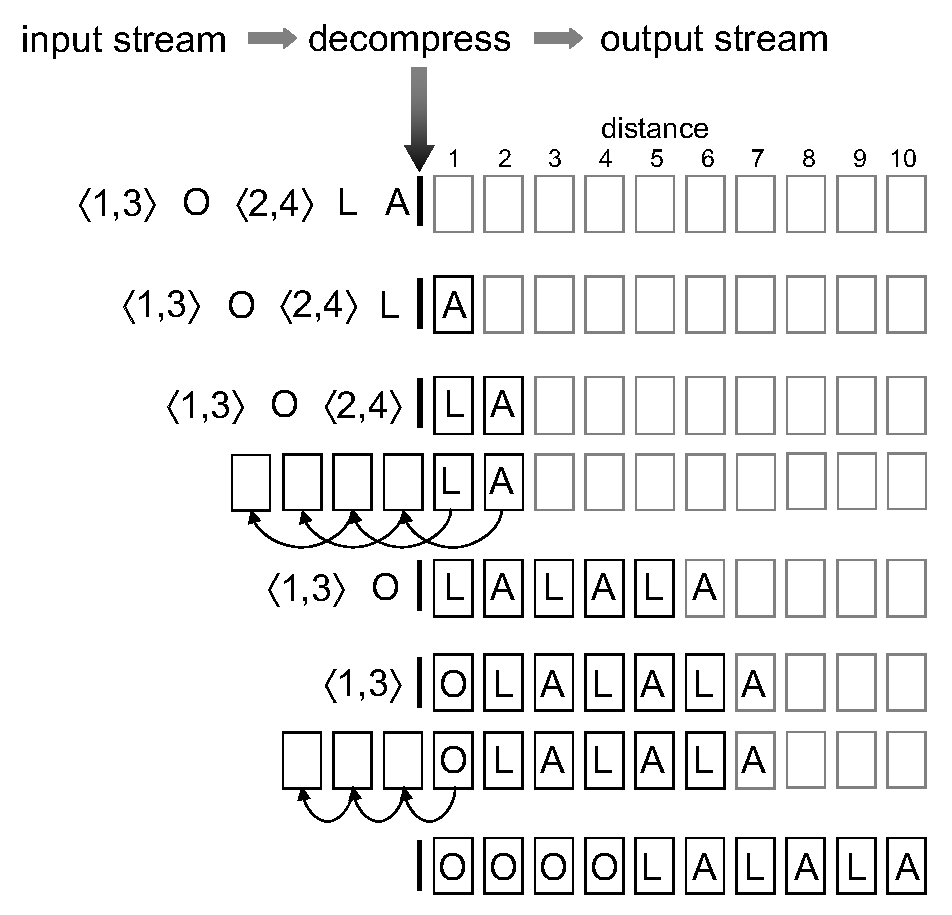
\psfig{file=compression/lz77-figure.eps,width=2.6in}
\caption{Example of LZ77 decompression.
\protect\label{fig:lz77}}
\end{figure}

%% \begin{figure}[t]
%% 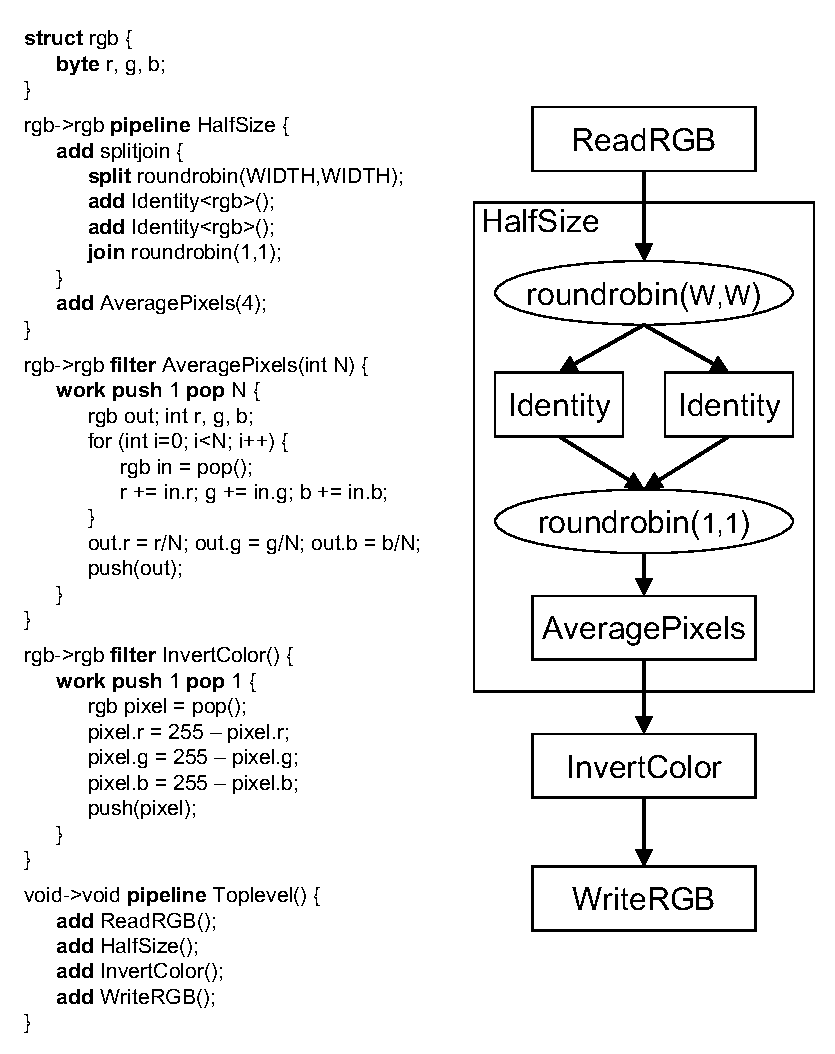
\psfig{file=compression/streamit-figure.eps,width=3.408in}
%% \caption{Example StreamIt program.
%% \protect\label{fig:streamit}}
%% \end{figure}

\section{Mapping into the Compressed Domain}

Our technique allows any cyclo-static dataflow program to operate
directly on LZ77-compressed data.  Rather than modifying the code
within the actors, our transformation treats actors as black boxes and
wraps them in a new execution layer.  The transformation attempts to
preserve as much compression as possible without ever performing an
explicit re-compression step.  While there exist cases in which the
output data will not be as compressed as possible, under certain
conditions the output is guaranteed to be fully compressed (relative
to the compression of the input).  We quantify this issue later.

To describe the mapping into the compressed domain, we consider each
StreamIt construct in turn.  Filters and joiners are described here,
while splitters are described in our technical
report~\cite{techreport}.

\newcommand{\mynewline}[0]{\\}
\begin{figure}[t]
\vspace{-6pt}
\centering
\begin{minipage}{0.62\textwidth}
{\it Execute a filter in the compressed domain, given that it consumes
  $n$ items and produces $m$ items on each execution.}\mynewline
\textsc{Execute-Compressed-Filter}~(int $n$, int $m$) \{\mynewline
\mbox{~~~~}{\bf while true} \{\mynewline
\mbox{~~~~}\mbox{~~~~}{\it /* pass-uncompressed */} \mynewline
\mbox{~~~~}\mbox{~~~~}{\bf if} input {\bf endswith} $n$ values {\bf then}\mynewline
\mbox{~~~~}\mbox{~~~~}\mbox{~~~~}{\bf execute} one call to uncompressed filter\mynewline
\mbox{~~~~}\mbox{~~~~}~\mynewline
\mbox{~~~~}\mbox{~~~~}{\it /* pass-compressed */} \mynewline
\mbox{~~~~}\mbox{~~~~}{\bf else if} input {\bf endswith} $\langle d,c \rangle$\mynewline
\mbox{~~~~}\mbox{~~~~}\mbox{~~~~~~~}{\bf and} $d\%n = 0$ {\bf and} $c \geq n$ {\bf then}\mynewline
\mbox{~~~~}\mbox{~~~~}\mbox{~~~~}{\bf replace} $\langle d,c \rangle$ with $\langle d, c\%n\rangle$ on input\mynewline
\mbox{~~~~}\mbox{~~~~}\mbox{~~~~}{\bf push} $\langle m~d/n, m~(c-c\%n)/n \rangle$ to output\mynewline
\mbox{~~~~}\mbox{~~~~}~\mynewline
\mbox{~~~~}\mbox{~~~~}{\bf else}\mynewline
\mbox{~~~~}\mbox{~~~~}\mbox{~~~~}{\bf let} $\langle d,c \rangle = $ last repeat on input\mynewline
\mbox{~~~~}\mbox{~~~~}\mynewline
\mbox{~~~~}\mbox{~~~~}\mbox{~~~~}{\it /* coarsen-repeat */}\mynewline
\mbox{~~~~}\mbox{~~~~}\mbox{~~~~}{\bf let} $L = \mbox{LCM}(d, n)$\mynewline
\mbox{~~~~}\mbox{~~~~}\mbox{~~~~}{\bf if} $d < L < c$ {\bf then} {\bf replace} $\langle d,c \rangle$\mynewline
\mbox{~~~~}\mbox{~~~~}\mbox{~~~~}\mbox{~~~~}\mbox{~~~~~}with $\langle c - (L - d) \rangle, \langle d, L - d\rangle$ on input\mynewline
\mbox{~~~~}\mbox{~~~~}\mynewline
\mbox{~~~~}\mbox{~~~~}\mbox{~~~~}{\it /* expand */}\mynewline
\mbox{~~~~}\mbox{~~~~}\mbox{~~~~}{\bf else if} $c > 0$ {\bf then}\mynewline
\mbox{~~~~}\mbox{~~~~}\mbox{~~~~}\mbox{~~~~}{\bf decode} $\langle d,c \rangle$ into $\langle d,c-1\rangle,V$ on input\mynewline
\mbox{~~~~}\mbox{~~~~}\mbox{~~~~}{\bf else}\mynewline
\mbox{~~~~}\mbox{~~~~}\mbox{~~~~}\mbox{~~~~}{\bf remove} $\langle d,c \rangle$ from input\mynewline
\mbox{~~~~}\}\mynewline
\}\mynewline
\end{minipage}
\vspace{-6pt}
\caption[Translation of filters into the compressed
  domain]{Translation of filters into the compressed domain.  We use
  $\%$ to denote a modulo operation.
%Helper functions appear in Figure~\ref{fig:helpers}.
\protect\label{fig:translate-filter}}
\end{figure}

\begin{figure}[t]
\centering
\vspace{-6pt}
\begin{minipage}{0.75\textwidth}
{\it Execute a roundrobin joiner in the compressed domain, given that
  it inputs $n_1$ items from input1 and $n_2$ items from input2 on
  each execution.}\mynewline
\textsc{Execute-Compressed-Joiner}~(int $n_1$, int $n_2$) \{\mynewline
\mbox{~~~~}{\bf while true} \{\mynewline \mbox{~~~~}\mbox{~~~~}{\it /*
  pass-uncompressed */}\mynewline \mbox{~~~~}\mbox{~~~~}{\bf if}
input1 {\bf endswith} value\mynewline
\mbox{~~~~}\mbox{~~~~}\mbox{~~~~}{\bf transfer} value from input1 to
output\mynewline \mbox{~~~~}\mbox{~~~~}\mynewline
\mbox{~~~~}\mbox{~~~~}{\it /* pass-compressed-long */}\mynewline
\mbox{~~~~}\mbox{~~~~}{\bf else if} input1 {\bf endswith} $\langle
d_1,c_1 \rangle$ {\bf and} $d_1\%n_1 = 0$\mynewline
\mbox{~~~~}\mbox{~~~~}\mbox{~~~~~~~}{\bf and} input2 {\bf endswith}
$\langle d_2,c_2 \rangle$ {\bf and} $d_2\%n_2 = 0$\mynewline
\mbox{~~~~}\mbox{~~~~}\mbox{~~~~~~~}{\bf and} $d_1/n_1 = d_2/n_2$ {\bf
  then}\mynewline \mbox{~~~~}\mbox{~~~~}\mbox{~~~~}{\bf let} $(L_1,
L_2)$ = \textsc{Repeat\_Lengths}($c_1$, $c_2$, {\it pos})\mynewline
\mbox{~~~~}\mbox{~~~~}\mbox{~~~~}{\bf replace} $\langle d_1, c_1
\rangle$ with $\langle d_1, c_1-L_1\rangle$ on input1\mynewline
\mbox{~~~~}\mbox{~~~~}\mbox{~~~~}{\bf replace} $\langle d_1, c_2
\rangle$ with $\langle d_2, c_2-L_2\rangle$ on input2\mynewline
\mbox{~~~~}\mbox{~~~~}\mbox{~~~~}{\bf push} $\langle d_1(n_1+n_2)/n_1,
L_1+L_2 \rangle$ to output\mynewline \mbox{~~~~}\mbox{~~~~}\mynewline
\mbox{~~~~}\mbox{~~~~}{\it /* pass-compressed-short */}\mynewline
\mbox{~~~~}\mbox{~~~~}{\bf else if} input1 {\bf endswith} $\langle
d_1,c_1 \rangle$ {\bf and} $c_1>0$\mynewline
\mbox{~~~~}\mbox{~~~~}\mbox{~~~~}{\bf let} offset = {\bf if} $d\%n_1
\leq \mbox{\it pos}$ {\bf then} {\it pos} {\bf else} $d\%n_1 +
n_2$\mynewline \mbox{~~~~}\mbox{~~~~}\mbox{~~~~}{\bf let} L = {\bf
  min}($c$, \textsc{Join\_Potential}($d$))\mynewline
\mbox{~~~~}\mbox{~~~~}\mbox{~~~~}{\bf replace} $\langle d, c\rangle$
with $\langle d, c - L\rangle$ on input1\mynewline
\mbox{~~~~}\mbox{~~~~}\mbox{~~~~}{\bf push} $\langle
(n_1+n_2)~\mbox{\bf floor}(d/n_1) + \mbox{offset}, L \rangle$ to
output\mynewline \mbox{~~~~}\mbox{~~~~}\mynewline
\mbox{~~~~}\mbox{~~~~}{\it /* prune */}\mynewline
\mbox{~~~~}\mbox{~~~~}{\bf else~} {\it /* input1 endswith}~$\langle
d_1, 0 \rangle$~{\it */}\mynewline
\mbox{~~~~}\mbox{~~~~}\mbox{~~~~}{\bf remove} $\langle d_1,0 \rangle$
from input1\mynewline \mbox{~~~~}\}\mynewline
\}\mynewline
\end{minipage}
\vspace{-6pt}
\caption[Translation of joiners into the compressed
  domain]{Translation of joiners into the compressed domain.  We use
  $\%$ to denote a modulo operation.
%Helper functions appear in Figure~\ref{fig:helpers}.
\protect\label{fig:translate-joiner}}
\end{figure}

\subsection*{Filters}

The procedure for translating a filter into the compressed domain is
given in Figure~\ref{fig:translate-filter}, and an example appears in
Figure~\ref{fig:filter-example}.  The behavior of the
compressed-domain filter can be considered in two pieces.  The first
piece consists of the simple case (annotated {\it pass-uncompressed}
in the code) in which the upcoming inputs to the filter are
uncompressed values.  In this case, the original filter is called with
those inputs, transforming $n$ input items to $m$ output items.  The
rest of the code deals with repeat tokens, attempting to translate
them across the filter with the minimum decompression needed.

The {\bf key idea behind our technique} is encapsulated in the {\it
  pass-compressed} case in Figure~\ref{fig:translate-filter}.  This
rule specifies how to translate a repeat token directly from a
filter's input tape to a filter's output tape without invoking the
filter's computation.  This translation is possible whenever the
repeat distance $d$ is a multiple of the filter's input rate $n$.  In
other words, the repeat is aligned with the execution boundaries of
the actor, so invoking the actor would produce the same results as
before.  In transferring the repeat token to the output tape, two
adjustments are made: 1) the distance and count are scaled by a factor
of $m/n$ to reflect possible differences between the output ($m$) and
input ($n$) rates of the actor, and 2) if the count is not an even
multiple of the input rate, then some leftover items ($c\%n$, where
$\%$ represents the modulo operation) are left on the input tape.

In cases where the repeat distance does not match the granularity of
the actor, the distance can sometimes be adjusted to allow
compressed-domain processing.  The {\it coarsen-repeat} rule
represents such an adjustment.  Consider that a filter inputs two
items at a time, but encounters a long repeat with distance three and
count 100.  That is, the input stream contains a regular pattern of
values with periodicity three.  Though consecutive executions of the
filter are aligned at different offsets in this pattern, every third
filter execution (spanning six values) falls at the same alignment.
In general, a repeat with distance $d$ can be exploited by a filter
with input rate $n$ by expanding the distance to $\mbox{LCM}(d, n)$.
In order to perform this expansion, the count must be greater than the
distance, as otherwise the repeat references old data that may have no
periodicity.  Also, the stream needs to be padded with $\mbox{LCM}-d$
values before the coarsened repeat can begin; this padding takes the
form of a shorter repeat using the original distance.

A second way to adjust a repeat token for compressed-domain processing
is by changing its count rather than its distance (rule {\it expand}).
The expand rule is invoked if a repeat has a count less than $n$, if
it is unaligned with the boundaries of an actor's execution, or if its
distance is not a multiple of $n$ (and cannot be coarsened
appropriately).  The expand rule decodes a single value from a repeat
token, thereby decreasing its count by one; the rest of the repeat may
become aligned later.  If the count of a repeat reaches zero, it is
eliminated.

Note that the {\it expand} rule requires partial decompression of the
data stream.  In order to perform this decompression, it may be
necessary to maintain an auxiliary data structure--separate from the
filter's input stream--that holds a complete window of decompressed
data.  This auxiliary structure is needed because the sliding-window
dictionary of LZ77 makes it difficult to decode one element without
decoding others.  However, even if the stream is fully decompressed in
parallel with the main computation, our technique retains many
benefits because the filters still operate on the compressed stream;
the volume of data processed is reduced, and the cost of
re-compression is averted.  For general algorithms such as gzip,
compression can be up to 10x slower than
decompression~\cite{ziviani00compression}.

%% The alignment stage sometimes needs to partially decompress the
%% data in the stream.  Due to the sliding-window dictionary in LZ77,
%% in general it is difficult to decode only a few items without
%% decompressing others.  Thus, our formulation assumes that a fully
%% decompressed version of the stream is available; the transition
%% rules access the decompressed data using the \mbox{\it decode}
%% function, which returns the sequence of values represented by a
%% repeat token at its current position in the stream.  However, in
%% practice, this decompression can be avoided whenever the repeat
%% distance is the same as the window size, as this simply causes a
%% value in the window to be overwritten by itself.  This case is very
%% common in several practical compression formats; for example, in
%% Apple Animation, the vast majority of repeats reference the same
%% pixel in the previous frame (which is also the window size), and
%% thus most decompression is avoided.  In run-length encoding, the
%% repeat distance and the window size are always equal to one, so no
%% decompression is needed.  While general LZ77 does require a
%% decompressed window to be maintained, our technique still offers
%% significant benefits by computing on a smaller volume of data and
%% avoiding the cost of re-compression.  For general algorithms such
%% as gzip, compression can be up to 10x slower than
%% decompression~\cite{ziviani00compression}.

\begin{figure*}[t]
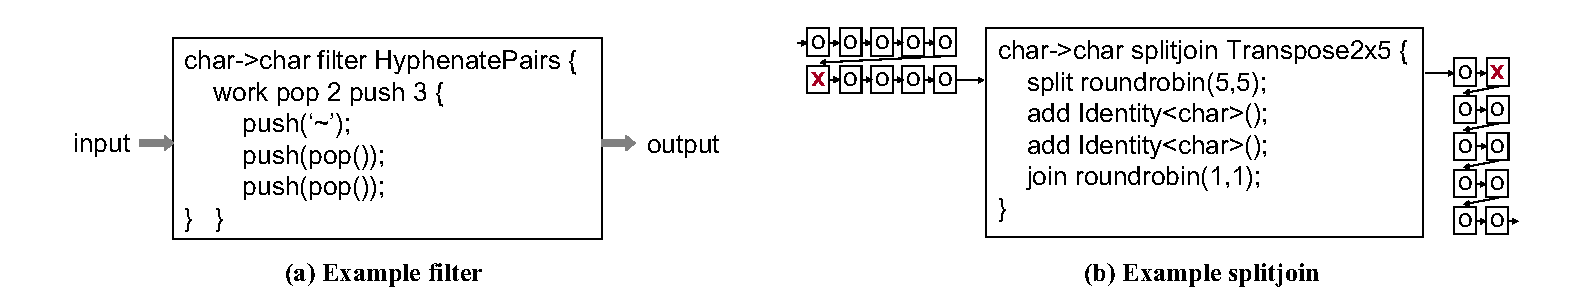
\psfig{file=compression/compressed-filters-in-streamit.eps,width=\textwidth}
\caption[Example StreamIt code to be mapped into the compressed
  domain]{Example filter, splitter, and joiner in StreamIt.  The
  splitter and joiner combine to form a Transpose. Translation to the
  compressed domain is illustrated in Figures~\ref{fig:filter-example}
  and~\ref{fig:sj-example}.\protect\label{fig:streamit-example}}
\end{figure*}

\begin{figure*}[t]
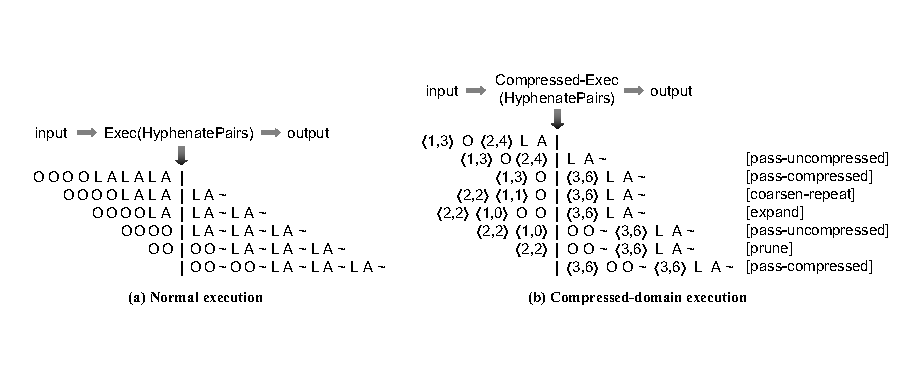
\psfig{file=compression/compressed-filter-example.eps,width=\textwidth}
\caption[Example execution of a filter in the uncompressed and
  compressed domains]{Example execution of a filter in the
  uncompressed and compressed domains.  See
  Figure~\ref{fig:streamit-example}(a) for the source
  filter.\protect\label{fig:filter-example}}
\end{figure*}

\subsection*{Joiners}

%% It is necessary to consider splitters and joiners separately from
%% general-purpose actors because of their pass-through semantics: the
%% inputs are distributed to the outputs without performing any
%% computation.  Our translation to the compressed domain leverages this
%% fact to preserve considerably more compression than would be possible
%% if splitters and joiners were viewed as opaque computational nodes
%% with multiple inputs and multiple outputs.

The procedure for executing a joiner in the compressed domain appears
in Figure~\ref{fig:translate-joiner}, while an example appears in
Figure~\ref{fig:sj-example}.  To simplify the presentation, we
consider a joiner with only two input streams.  This captures all of
the fundamental ideas; extension to additional streams is
straightforward.  In addition, we use the following notations:

\begin{figure*}[t]
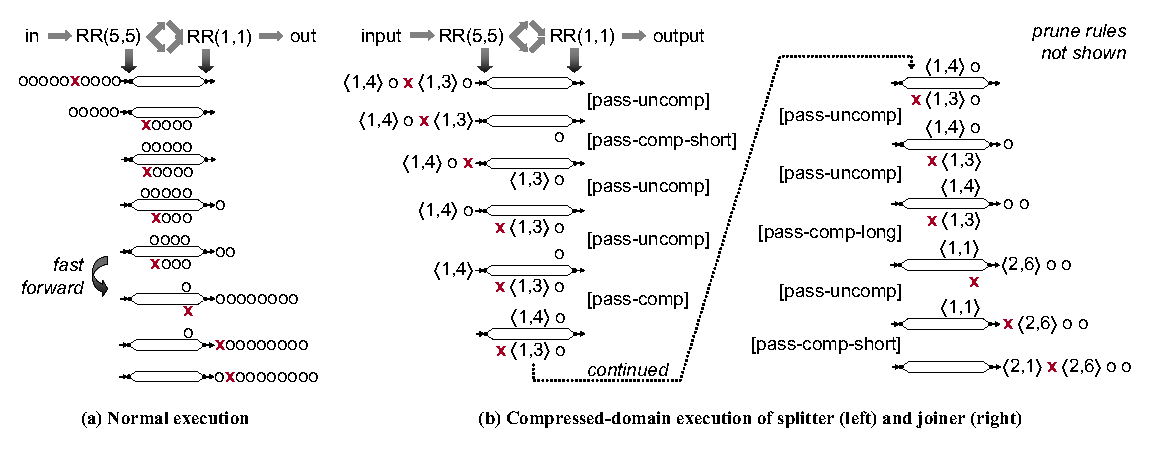
\psfig{file=compression/compressed-splitjoin-example.eps,width=\textwidth}
\caption[Example execution of splitters and joiners in the compressed
  domain]{Example execution of splitters and joiners in the compressed
  domain.  As illustrated by the input/output pairs in
  Figure~\ref{fig:streamit-example}(b), the example performs a
  transpose of a 2x5 matrix.  When the matrix is linearized as shown
  here, the input stream traverses the elements row-wise while the
  output stream traverses column-wise.  Due to redundancy in the
  matrix, this reordering can be done largely in the compressed
  domain.  \protect\label{fig:sj-example}}
\end{figure*}

\begin{itemize}

\item Splitters and joiners adopt a fine-grained cyclo-static
  execution model, in which each execution step transfers only one
  item from an input tape to an output tape.  That is, a
  roundrobin$(n_1, n_2)$ joiner has $n_1 + n_2$ distinct execution
  steps.  We refer to every group of $n_1 + n_2$ steps as an {\it
    execution cycle}.

\item The pseudocode in Figure~\ref{fig:translate-joiner} assumes,
  without loss of generality, that the next execution step of the
  joiner will read from the first input stream (input1).

\item We use $\pos$ to denote the number of items (in terms of the
  uncompressed domain) that have already been read from the current
  input stream (input1) in the current execution cycle.  For brevity,
  the pseudocode does not maintain the value of $\pos$, though it is
  straightforward to do so.

\end{itemize}

\begin{figure}[t]
\centering
\begin{minipage}{0.75\textwidth}
{\it Given that $c_1$ and $c_2$ compressed items are available on the
  first and second input streams of a joiner, returns the number of
  items that can be read from each input before one of them is
  exhausted.  Assumes that the joiner is currently reading from the
  first input stream, from which \mbox{pos} items have previously been
  consumed in the current execution cycle.}\\
\textsc{Repeat\_Lengths}$(c_1, c_2, \pos )$~returns~(int,~int)~\{\\
\tab{\it // the number of complete joiner cycles, and the leftovers}\\
\tab$\mbox{total\_cycles} = \mbox{floor}(c/(n_1 + n_2))$\\
\tab$\mbox{leftover}_1 = c_1 - \mbox{total\_cycles} * n_1$\\
\tab$\mbox{leftover}_2 = c_2 - \mbox{total\_cycles} * n_2$\\
~ \vspace{-6pt}\\
\tab{\it // the last partial cycle may end in three regions:}\\
\tab$\mbox{\bf if~} \mbox{leftover}_1 \leq n_1 - \pos$~\{\\
\tab\tab{\it // 1. in reading from the first input stream}\\
\tab\tab$L_1 = \mbox{leftover}_1$\\
\tab\tab$L_2 = 0$\\
\tab$\} \mbox{\bf~else if~} \mbox{leftover}_2 \leq n_2~\{$\\
\tab\tab{\it // 2. in subsequent reading from the second input stream}\\
\tab\tab$L_1 = n_1-\pos$\\
\tab\tab$L_2 = \mbox{leftover}_2$\\
\tab\} \mbox{\bf ~else} \{\\
\tab\tab{\it // 3. in wrap-around reading from the first input stream}\\
\tab\tab$L_1 = \mbox{leftover}_1$\\
\tab\tab$L_2 = n_2$\\
\tab\}\\
~ \vspace{-6pt}\\ 
\tab$\mbox{\bf return~}(n_1*\mbox{total\_cycles} + L_1, n_2*\mbox{total\_cycles} + L_2)$
\}
\end{minipage}
\caption[\textsc{Repeat\_Lengths} function for compressed joiner
  execution]{The \textsc{Repeat\_Lengths} function is called during
  compressed joiner execution.  In the case where the input tokens to
  the joiner have compatible repeat distances, it calculates the
  maximum repeat lengths that can be passed to the
  output.\protect\label{fig:repeat-lengths}}
\end{figure}

There are two ways to pass repeat tokens through a joiner.  If the
input streams contain compatible repeat tokens, then they can be
combined into a long repeat that spans multiple execution cycles;
otherwise, a shorter repeat is extracted from only one of the streams.

The first and most powerful way to execute joiners in the compressed
domain is to combine repeat tokens from both input streams (case {\it
  pass-compressed-long} in Figure~\ref{fig:translate-joiner}).  For this to
be possible, both repeat distances must be the same multiple of their
respective joiner weight ($n_1$ or $n_2$); the combined token has a
repeat distance that is a multiple of $n_1 + n_2$.  The
\textsc{Repeat\_Lengths} routine (detailed in
Figure~\ref{fig:repeat-lengths}) calculates the maximum repeat length
depending on the current position of the joiner and the repeat lengths
of the inputs.

The second mode of compressed joiner execution ({\it
  pass-compressed-short}) inputs only a single repeat token,
extracting the maximum length that can safely move to the output.  The
\textsc{Join\_Potential} routine (detailed in
Figure~\ref{fig:join-potential}) determines how much of the repeat can
be moved to the output before the data referenced would have
originated from a different input stream.

\section{Supported File Formats}
\label{sec:formats}

As LZ77 refers to a compression algorithm rather than a complete
compression format, there are additional factors to consider in
mapping computations to real-world image and video codecs.  Some
codecs are a subset of LZ77, utilizing only run-length encoding or a
fixed window size; these are supported very efficiently by our
technique.  Others are a superset of LZ77, incorporating additional
techniques such as delta coding or Huffman coding; these may incur
additional processing overhead.  In the following sections, we
describe the practical considerations involved in targeting various
compression formats with our technique.  Formats are ordered by
approximate goodness of the achievable mapping.

\subsection*{High-Efficiency Mappings}
\label{sec:formats-good}

All of the formats in this category can be considered to be subsets of
LZ77.

\begin{enumerate}

\item {\it Apple Animation.}  The Apple Animation codec (which forms
  the basis for our experimental evaluation) is supported as part of
  the Quicktime MOV container format.  It serves as an industry
  standard for exchanging computer animations and digital video
  content before they are rendered to lossy formats for final
  distribution~\cite[p.~106]{adobe-anim}\cite[p.~284]{harrington-anim}
  \cite[p.~367]{long-anim}\cite[p.~280]{pogue-anim}.

The Animation codec represents a restricted form of LZ77 in which
repeat distances are limited to two values: a full frame or a single
pixel.  A repeat across frames indicates that a stretch of pixels did
not change from one frame to the next, while a repeat across pixels
indicates that a stretch of pixels has the same color within a frame.
% mention bit depths?

\item {\it Flic Video.}
Flic Video files (FLI/FLC) were originally produced by Autodesk
Animator and are still supported by many animation packages today.
Their compression of frame data is almost identical to Apple
Animation.

\begin{figure}[t]
\centering
\begin{minipage}{0.75\textwidth}
{\it Given a repeat token with distance $d$ on the current input
  stream of a joiner, returns the maximum count of a repeat token that
  could safely be emitted to the output stream.  Assumes that only a
  single repeat token is available (i.e., the {\tt
    pass-compressed-long} rule does not apply).}
\textsc{Join\_Potential}$(d)$~returns~int~\{\\ \tab$\mbox{offset} =
d$\%$n_1$\\ \tab$\mbox{{\bf if~}} \mbox{offset} \leq \pos
~\{$\\ \tab\tab{\it // repeat for remainder of this execution
  cycle}\\ \tab\tab$\mbox{\bf return~} n_1 - \pos$\\ \tab$\} \mbox{\bf
  ~else} ~\{$\\ \tab\tab{\it // repeat until referenced data goes out
  of range}\\ \tab\tab$\mbox{\bf return~} \mbox{offset} -
\pos$\\ \tab$\}$\\ \}
\end{minipage}
\caption[\textsc{Join\_Potential} function for compressed joiner
  execution]{The \textsc{Join\_Potential} function is called during
  compressed joiner execution.  In the case where the input tokens to
  the joiner have incompatible repeat distances, it calculates the
  maximum length of the current token that may be passable to the
  output. \protect\label{fig:join-potential}}
\end{figure}

\item {\it Microsoft RLE.}  Microsoft RLE compression can appear in
  both BMP images and AVI animations.  Apart from bit-depth and
  formatting details, its capabilities are identical to Apple
  Animation; it can perform run-length encoding within a frame, and
  can skip over pixels to exploit inter-frame redundancy.

\item {\it Targa.} The Truevision Targa (TGA) format is a simple image
  format that is widely used to render frame sequences in the computer
  animation and video industries.  The format includes an optional RLE
  compression stage, making it a good target for our technique.

\item {\it PXY.} The pxy format is a research-based image format
  designed to support efficient transpose and rotation of
  black-and-white images~\cite{shoji95}.  It consists of the series of
  $(x,y)$ coordinates at which the image changes color during a
  horizontal scan.  As this information can be converted to a
  run-length encoding, it can also be targeted by our technique.

\end{enumerate}

\subsection*{Medium-Efficiency Mappings}
\label{sec:formats-med}

While the formats in this category utilize an encoding that is
compatible with LZ77, they incur extra overhead because the data is
reorganized prior to the compression stage.

\begin{enumerate}

\item {\it Planar RGB.} The Planar RGB video format is supported by
  Apple Quicktime files.  It utilizes run-length encoding for pixels
  within a frame, with partial support for expressing inter-frame
  repeats (only the end of lines can be skipped).  The red, green, and
  blue planes are encoded separately in order to increase compression.
  For user transformations that need to process red, green, and blue
  values together, this introduces additional alignment overhead when
  applying our technique.

\item {\it OpenEXR.} OpenEXR is an emerging image format (backed by
  Industrial Light and Magic) for use in digital film.  It offers
  several compression options, including run-length encoding, zip, and
  wavelet-based compression.  However, in run-length encoding mode,
  the low and high bytes of the pixels are separated and encoded as
  separate run-length sequences; this enables pixels with variations
  in the low bytes to nonetheless benefit from compression of the high
  bytes.  As most user transformations would utilize the entire
  bit-width of the pixel, our technique suffers additional alignment
  overhead in processing these files.

\end{enumerate}

\subsection*{Low-Efficiency Mappings}
\label{sec:formats-bad}

The formats in this category are supersets of LZ77.  While our
technique could offer some gains in exploiting the LZ77 compression,
it would have to undo any compression sitting on top of LZ77 and
offers limited benefit for filters (as in PNG) applied underneath
LZ77.

\begin{enumerate}

\item {\it DEFLATE.}  DEFLATE is a general-purpose algorithm that
  provides all of the compression for popular formats such as ZIP and
  GZIP.  The algorithm consists of a full LZ77 encoder followed by
  Huffman coding, which resizes the symbols in the stream to match
  their usage frequencies.  In targeting ZIP or GZIP with our
  transformations, we would first have to undo the Huffman coding
  (unless the application simply reordered data, in which case the
  coding could remain intact).  Though Huffman decoding is a
  lightweight lookup operation, it would also increase the memory
  footprint.  In addition, as DEFLATE's LZ77 algorithm operates on
  individual bytes, there may be an exaggerated alignment cost if the
  application operates on a larger word size.

\item {\it TSCC.}  The TechSmith Screen Capture Codec is very similar
  to Microsoft RLE, except that the final output is further compressed
  using DEFLATE.  Thus, any overheads incurred by our technique on
  DEFLATE also extend to TSCC.

\item {\it PNG.}  The PNG image format also relies on DEFLATE to
  compress the pixels in the image.  However, before running DEFLATE,
  the pixels are usually filtered with a delta encoding; each pixel is
  replaced with the difference between its value and a predicted
  value, where the prediction is a linear combination of neighboring
  pixels.  While program segments that compute a linear
  function~\cite{aalamb} could perhaps be mapped to this compressed
  format, our current technique only applies if the delta encoding is
  turned off.  Even in this scenario, there is a large amount of
  overhead due to the Huffman coding in DEFLATE.

\end{enumerate}

\begin{table*}[t]
\hspace{-0.26in}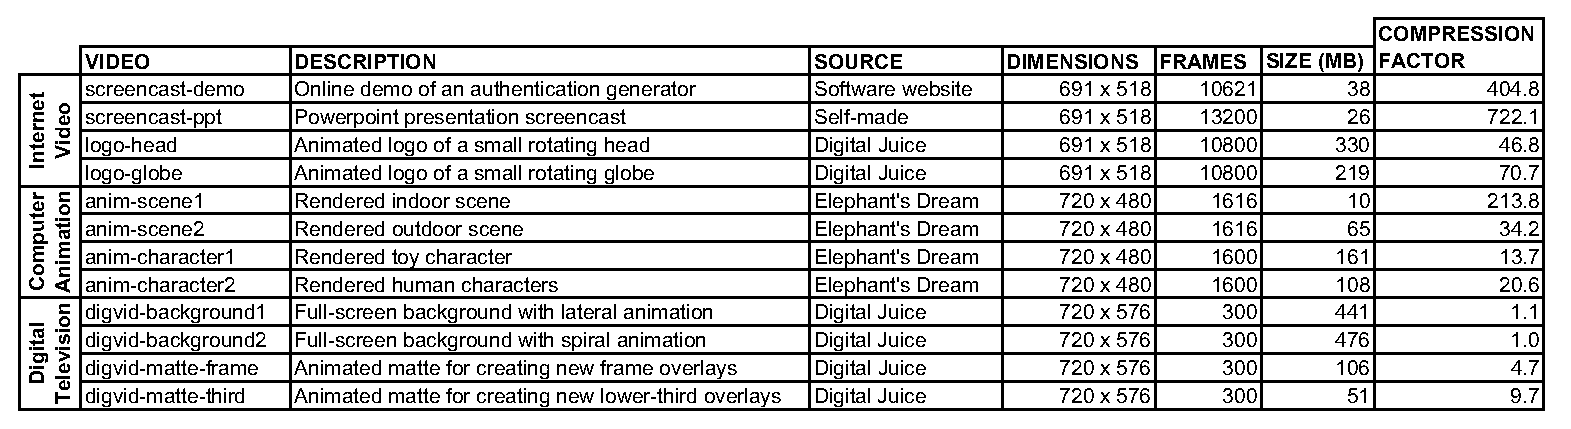
\psfig{file=compression/table-benchmarks.eps,width=7.02in}
\caption{Characteristics of the video workloads.
\protect\label{tab:videos}}
\end{table*}

\section{Experimental Evaluation}

To demonstrate the potential benefits of mapping into the compressed
domain, we implemented a few of our transformations as part of the
StreamIt compiler.  Our current implementation supports two
computational patterns: 1) transforming each individual element of a
stream (via a pop-1, push-1 filter), and 2) combining the elements of
two streams (via a roundrobin(1,1) joiner and a pop-2, push-1 filter).
The program can contain any number of filters that perform arbitrary
computations, so long as the I/O rates match these patterns.  While we
look forward to performing a broader implementation in future work,
these two building blocks are sufficient to express a number of useful
programs and to characterize the performance of the technique.

Our evaluation focuses on applications in digital video editing.
Given StreamIt source code that operates on pixels from each frame of
a video, the StreamIt compiler maps the computation into the
compressed domain and emits executable plugins for two popular video
editing tools, MEncoder and Blender.  The plugins are written for the
Apple Animation format (see Section~\ref{sec:formats-good}).

Our benchmarks fall into two categories: 1) pixel transformations,
such as brightness, contrast, and color inversion, which adjust pixels
within a single video, and 2) video compositing, in which one video is
combined with another as an overlay or mask.

The main results of our evaluation are:
\begin{itemize}

\item Operating directly on compressed data offers a speedup roughly
proportional to the compression factor in the resulting video.

\item For pixel transformations, speedups range from 2.5x to 471x,
  with a median of 17x.  Output sizes are within 0.1\% of input sizes
  and about 5\% larger (median) than a full re-compression.

\item For video compositing, speedups range from 1.1x to 32x, with a
  median of 6.6x.  Output files retain a sizable compression ratio
  (1.0x to 44x) and are about 52\% larger (median) than a full
  re-compression.

\end{itemize}
The following sections provide more details on our video workloads,
the evaluation of pixel transformations, and the evaluation of video
compositing.

\subsection*{Video Workloads}

Our evaluation utilizes a suite of 12 video workloads that are
described in Table~\ref{tab:videos}; some of the videos are also
pictured in Figure~\ref{fig:videos}.  The suite represents three
common usage scenarios for lossless video formats: Internet
screencasts, computer animation, and digital television production.
While videos in each area are often rendered to a lossy format for
final distribution, lossless codecs are preferred during the editing
process to avoid accumulating compression artifacts.  All of our
source videos are in the Apple Animation format (described in
Section~\ref{sec:formats-good}), which is widely used by video editing
professionals~\cite[p.~106]{adobe-anim} \cite[p.~284]{harrington-anim}
\cite[p.~367]{long-anim} \cite[p.~280]{pogue-anim}.  The Apple
Animation format is also popular for capturing video from the screen
or camera, as the encoder is relatively fast.

Our suite of videos is assembled from a variety of realistic and
industry-standard sources.  The first screencast is an online demo of
an authentication generator for rails~\cite{auth-demo}; the second is
a PowerPoint presentation (including animations), captured using
Camtasia Studio.  As Internet content is often watermarked with a logo
or advertisement, we include two animated logos in the ``Internet
video'' category.  These logos are taken from Digital
Juice~\cite{digital-juice}, a standard source for professional
animations, and rendered to Apple Animation format using their
software.  The animated logos are rendered full-frame (with the logo
in the corner) because compositing operations in our testbed (Blender)
are done on equal-sized videos.

The computer animation clips are derived from Elephant's Dream, a
short film with entirely open-source content~\cite{elephants-dream};
our videos are rendered from source using Blender.  Finally, the
digital television content is also taken from a Digital Juice
library~\cite{digital-juice}.  The backgrounds represent
high-resolution, rotating backdrops as might appear in the
introduction to a program.  The mattes are black-and-white animations
that can be used to synthesize a smaller overlay (such as a frame or a
``lower third'', often used for text) from a full animated background
(see Figure~\ref{fig:videos}b for an example).

The videos exhibit a wide range of compression factors.  The
screencasts have very high compression ($\sim$400x-700x) because only
a small part of the screen (e.g., a mouse, menu, or PowerPoint bullet)
is changing on any given frame; the Apple Animation format compresses
the inter-frame redundancy.  The compression for {\tt anim-scene1} is
also in excess of 200x because motion is limited to a small animated
character.  The animated logos are the next most compressed
($\sim$50-70x), influenced largely by the constant blank region
outside the logo.  The computer animation content ($\sim$10-30x
compression) has a high level of detail but benefits from both
inter-frame and intra-frame redundancy, as some rendered regions have
constant color.  Next are the digital video mattes ($\sim$5-10x
compression), which have fine-grained motion in some sections.
Finally, the digital video backgrounds offer almost no compression
gains (1.0-1.1x) under Apple Animation, as they have pervasive motion
and detail across the entire frame.

The Apple Animation format supports various bit depths.  All of our
source videos use 32 bits per pixel, allocating a single byte for each
of the red, green, blue, and alpha channels.

\subsection*{Pixel Transformations}

The pixel transformations adjust the color of each pixel in a uniform
way.  We evaluated three transformations:
\begin{itemize}
\item Brightness adjustment, which increases each RGB value by a value
of 20 (saturating at 255).
\item Contrast adjustment, which moves each RGB value away from the
center (128) by a factor of 1.2 (saturating at 0 and 255).

\item Color inversion, which subtracts each RGB value from 255 (useful
  for improving the readability of screencasts or for reversing the
  effect of video mattes).

\end{itemize}

We implemented each transformation as a single StreamIt filter that
transforms one pixel to another.  Because the filter has a pop rate of
one, it does not incur any alignment overhead.

\paragraph*{Setup}  The pixel transformations were compiled into plugins for
MEncoder, a popular command-line tool (bundled with MPlayer) for video
decoding, encoding, and filtering.  MEncoder relies on the FFMPEG
library to decode the Apple Animation format; as FFMPEG lacked an
encoder for this format, the authors implemented one.  Additionally,
as MEncoder lacks an interface for toggling only brightness or
contrast, the baseline configuration was implemented by the authors.

The baseline configuration performs decompression, pixel
transformations, then re-compression.  Because the main video frame is
updated incrementally by the decoder, the pixel transformations are
unable to modify the frame in place (otherwise pixels present across
frames would be transformed multiple times).  Thus, the baseline
transformation writes to a separate location in memory.  The optimized
configuration performs pixel transformations directly on the
compressed data, avoiding data expansion implied by decompression and
multiple frame buffers, before copying the data to the output file.

\begin{table*}[t]
\hspace{-0.26in}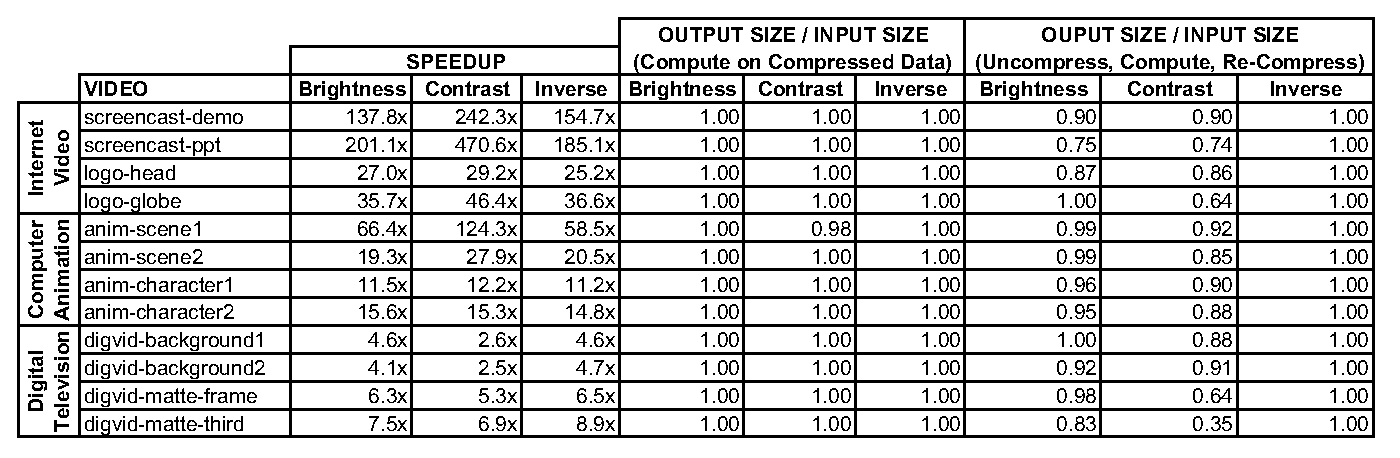
\psfig{file=compression/table-pixel-speedup.eps,width=7.02in}
\caption[Table of results for pixel transformations]{Results for pixel transformations.
\protect\label{tab:pixel-speedup}}
\end{table*}

Our evaluation platform is a dual-processor Intel Xeon (2.2 GHz) with
2 GB of RAM.  As all of our applications are single-threaded, the
second processor is not utilized.  For the timing measurements, we
execute each program five times and report the median user time.

\paragraph*{Results}  Detailed results for the pixel transformations appear
in Table~\ref{tab:pixel-speedup}.  Figure~\ref{fig:pixel-speedup}
illustrates the speedups, which range from 2.5x to 471x.  As
illustrated in Figure~\ref{fig:speedup-scatter}, the speedups are
closely correlated with the compression factor in the original video.
For the highly-compressed screencasts and {\tt anim-scene1}, speedups
range from 58x to 471x.  For the medium-compression computer
animations (including the animated logos), speedups range from 11x to
46x.  And for the low-compression digital television content, speedups
range from 2.5x to 8.9x.

There are two distinct reasons for the speedups observed.  First, by
avoiding the decompression stage, computing on compressed data reduces
the volume of data that needs to be stored, manipulated, and
transformed.  This savings is directly related to the compression
factor and is responsible for the upwards slope of the graph in
Figure~\ref{fig:speedup-scatter}.  Second, computing on compressed
data eliminates the algorithmic complexity of re-compression.  For the
Apple Animation format, the cost of compressing a given frame does not
increase with the compression factor (if anything, it decreases as
fewer pixels need a fine-grained encoding).  Thus, the baseline
devotes roughly constant runtime to re-compressing each video, which
explains the positive intercept in the graph of
Figure~\ref{fig:speedup-scatter}.

The impact of re-compression is especially evident in the digital
television examples.  Despite a compression factor of 1.0 on {\tt
digvid-background2}, our technique offers a 4.7x speedup on color
inversion.  Application profiling confirms that 
% NOTE: I profiled the hand-coded version rather than the StreamIt
% version.  It had a speedup of 5.5x rather than 4.7x
73\% of the baseline runtime is spent in the encoder; as this stage is
absent from the optimized version, it accounts for $1/(1-0.73) = 3.7$x
of the speedup.  The remaining speedup in this case is due to the
extra frame buffer (and associated memory operations) in the
decompression stage of the baseline configuration.
%
%(Don't really understand these profiling numbers yet)
%
%Note that videos with larger compression ratios spend
%a smaller fraction of time in the encoder; for example, color
%inversion on {\tt screencast1-demo} spends only 5\% of its time in the
%encoder (and 65\% of the time doing the transformation itself).

Another important aspect of the results is the size of the output
files produced.  Apart from the first frame of a video\footnote{In the
Apple Animation format, the first frame is encoded as if the previous
frame was black.  Thus, adjusting the color of black pixels in the
first frame may increase the size of the file, as it removes
inter-frame redundancy.}, performing pixel transformations directly on
compressed data will never increase the size of the file.  This is
illustrated in the middle columns of Table~\ref{tab:pixel-speedup}, in
which the output sizes are mostly equal to the input sizes (up to 2
decimal places).  The only exception is contrast adjustment on {\tt
anim-scene1}, in which the output is 2\% smaller than the input due to
variations in the first frame; for the same reason, some cases
experience a 0.1\% increase in size (not visisble in the table).

\begin{figure}[t]
\centering
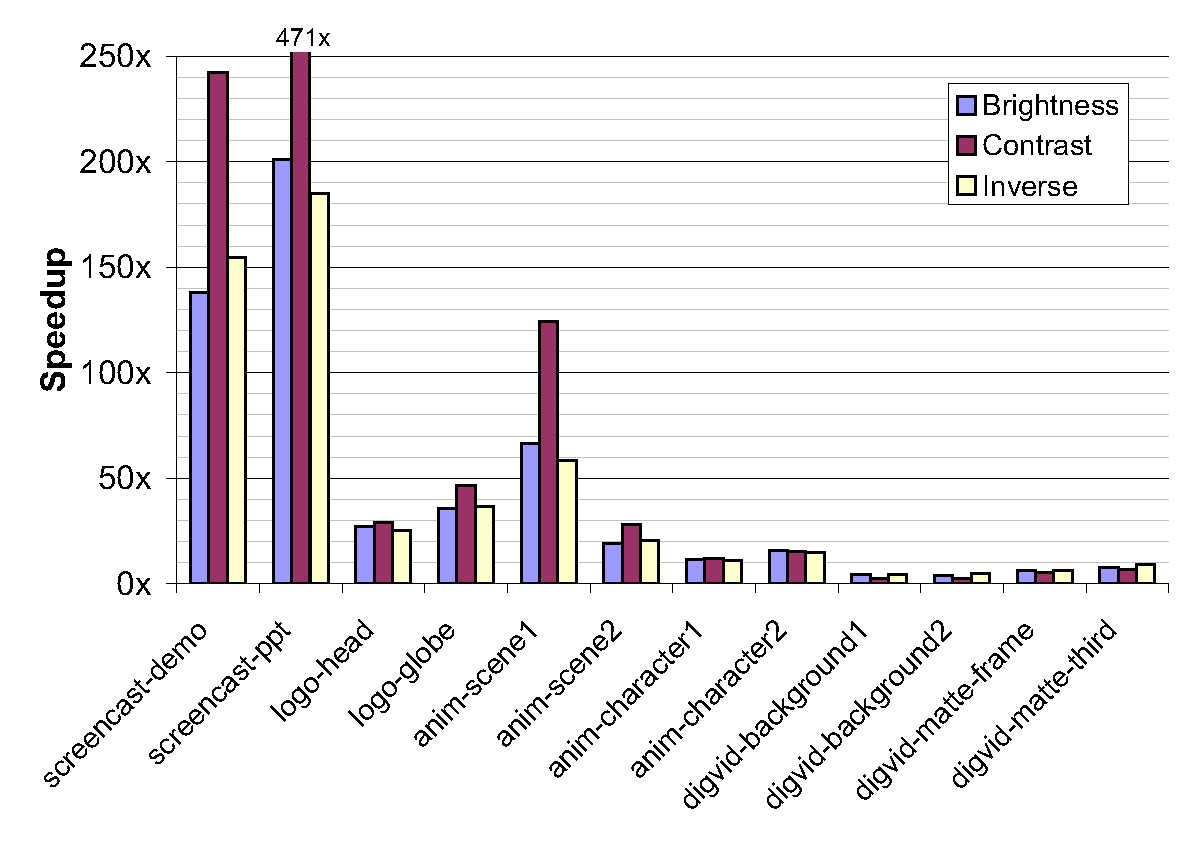
\psfig{file=compression/graph-speedup-pixel.eps,width=4.355in}
\caption[Speedup graph for pixel transformations]{Speedup on pixel transformations.
\protect\label{fig:pixel-speedup}}
\end{figure}

Though computing on compressed data has virtually no effect on the
file size, there are some cases in which the pixel transformation
increases the redundancy in the video and an additional re-compression
step could compress the output even further than the original input.
This potential benefit is illustrated in the last three columns of
Table~\ref{tab:pixel-speedup}, which track the output size of the
baseline configuration (including a re-compression stage) versus the
original input.  For the inverse transformation, no additional
compression is possible because inverse is a 1-to-1 transform: two
pixels have equal values in the output file if and only if they have
equal values in the input file.  However, the brightness and contrast
transformations may map distinct input values to the same output
value, due to the saturating arithmetic.  In such cases, the
re-compression stage can shrink the file to as low as 0.75x
(brightness) and 0.35x (contrast) its original size.  These are
extreme cases in which many pixels are close to the saturating point;
the median re-compression (across brightness and contrast) is only
10\%.

To achieve the minimal file size whenever possible, future work will
explore integrating a lightweight re-compression stage into the
compressed processing technique.  Because most of the compression is
already in place, it should be possible to improve the compression
ratio without running the full encoder (e.g., run-length encoded
regions can be extended without being rediscovered).  

% (The following comment didn't make sense -- to do the full
% re-compression, you would need to start from a decompressed stream,
% which has the full data volume.)
%
% Even running the full encoding algorithm (in place on the compressed
% data) may leave us with significant speedups, as much of the
% improvement comes from decreased data volume rather than decreased
% re-compression cost.

\subsection*{Video Compositing}

In video compositing, two videos are combined using a specific
function to derive each output pixel from a pair of input pixels (see
Figure~\ref{fig:videos}).  In the case of subtitling, animated logos,
and computer graphics, an alpha-under transformation is common; it
overlays one video on top of another using the transparency
information in the alpha channel.  In applying an animated matte, the
videos are combined with a multiply operation, thereby masking the
output according to the brightness of the matte.  For our experiments,
we generated composites using each foreground/background pair within a
given application area, yielding a total of 12 composites.

In StreamIt, we implemented each compositing operation as a
roundrobin(1,1) joiner (to interleave the streams) followed by a
filter (to combine the pixel values).  The intuition of the
compressed-domain execution is that if both streams have the same kind
of repeat (inter-frame or intra-frame), then the repeat is copied
directly to the output.  If they have different kinds of repeats, or
if one stream is uncompressed, then both streams are uncompressed.

\paragraph*{Setup} The compositing operations were compiled into plugins for
Blender, a popular tool for modeling, rendering, and post-processing
3-D animations.  Blender has logged 1.8 million downloads in the last
year~\cite{blender-stats} and was used in the production of Spiderman
2~\cite{blender-wikipedia}.  Like MEncoder, Blender relies on the
FFMPEG library for video coding, so we utilize the same Apple
Animation decoder/encoder as in the pixel transformations.

As Blender already includes support for video compositing, we use its
implementation as our baseline.  The compositing operations have
already been hand-tuned for performance; the implementation of
alpha-under includes multiple shortcuts, unrolled loops, and the
following comment: ``this complex optimalisation is because the
'skybuf' can be crossed in''.  We further improved the baseline
performance by patching other parts of the Blender source base, which
were designed around 3-D rendering and are more general than needed
for video editing.  We removed two redundant vertical flips for each
frame, two redundant BGRA-RGBA conversions, and redundant memory
allocation/deallocation for each frame.
% did not mention removal of O(frames^2) linked list search, although 
% this fell out of removing the redundant memory deallocation

\begin{figure}[t]
\centering
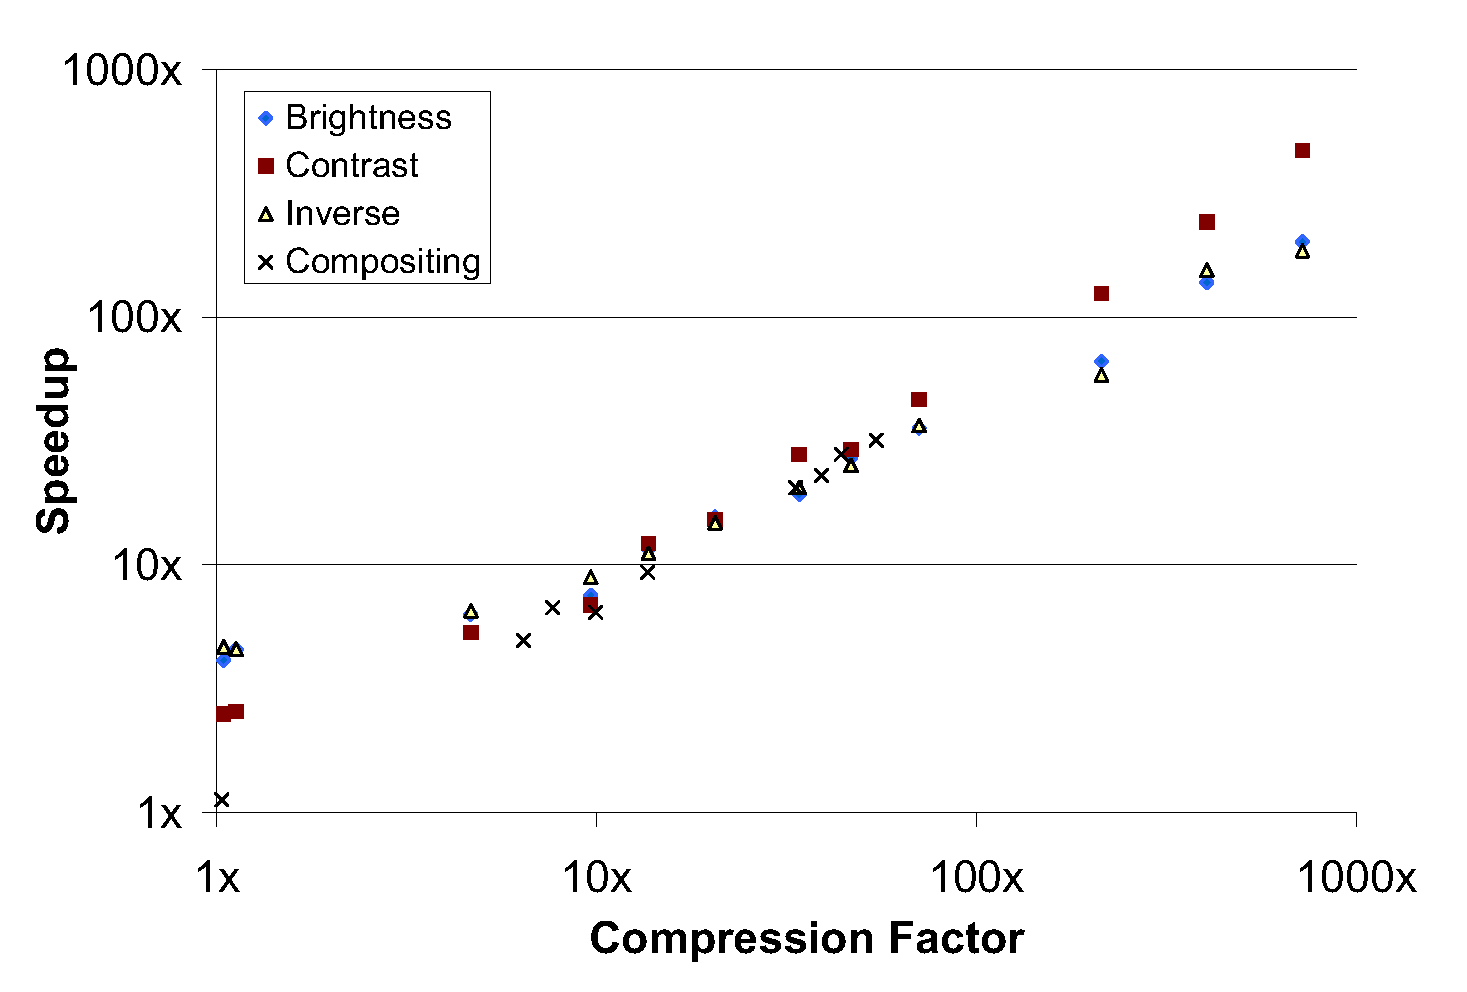
\psfig{file=compression/graph-speedup-scatter.eps,width=4.511in}
\caption{Speedup vs. compression factor for all transformations.
\protect\label{fig:speedup-scatter}}
\end{figure}

\begin{figure}[t]
\centering
\begin{minipage}{0.3\textwidth}
\centering
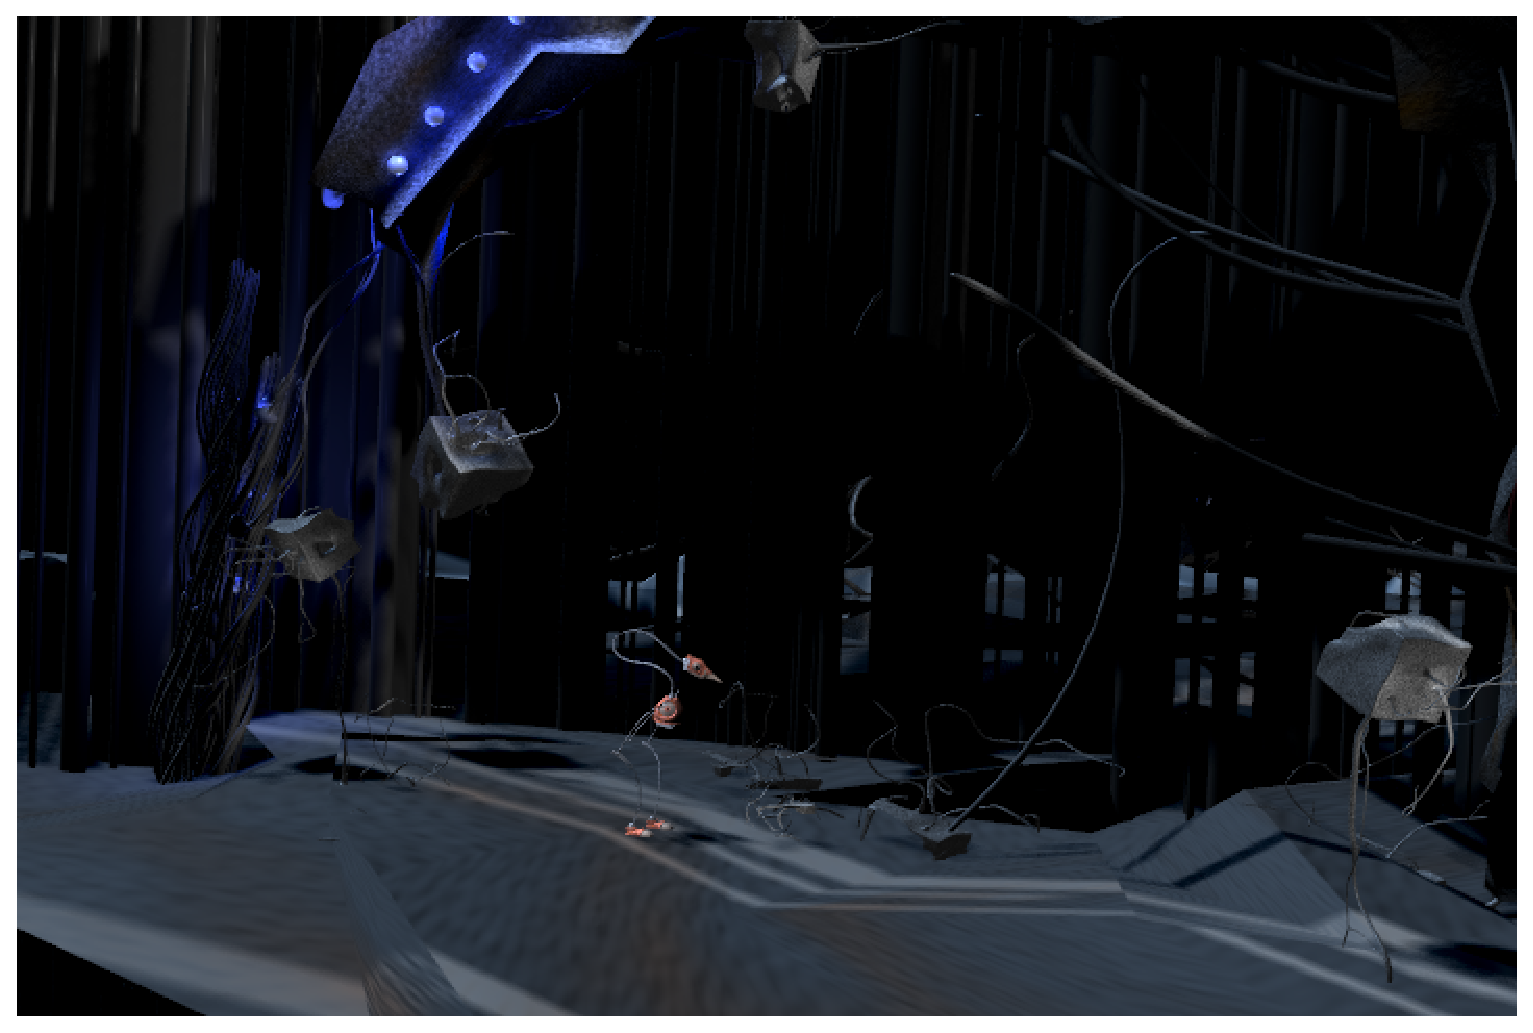
\psfig{file=compression/blender-background1-frame5.eps,width=1.9in}
\vspace{2pt}
\end{minipage}
\begin{minipage}{0.3\textwidth}
\centering
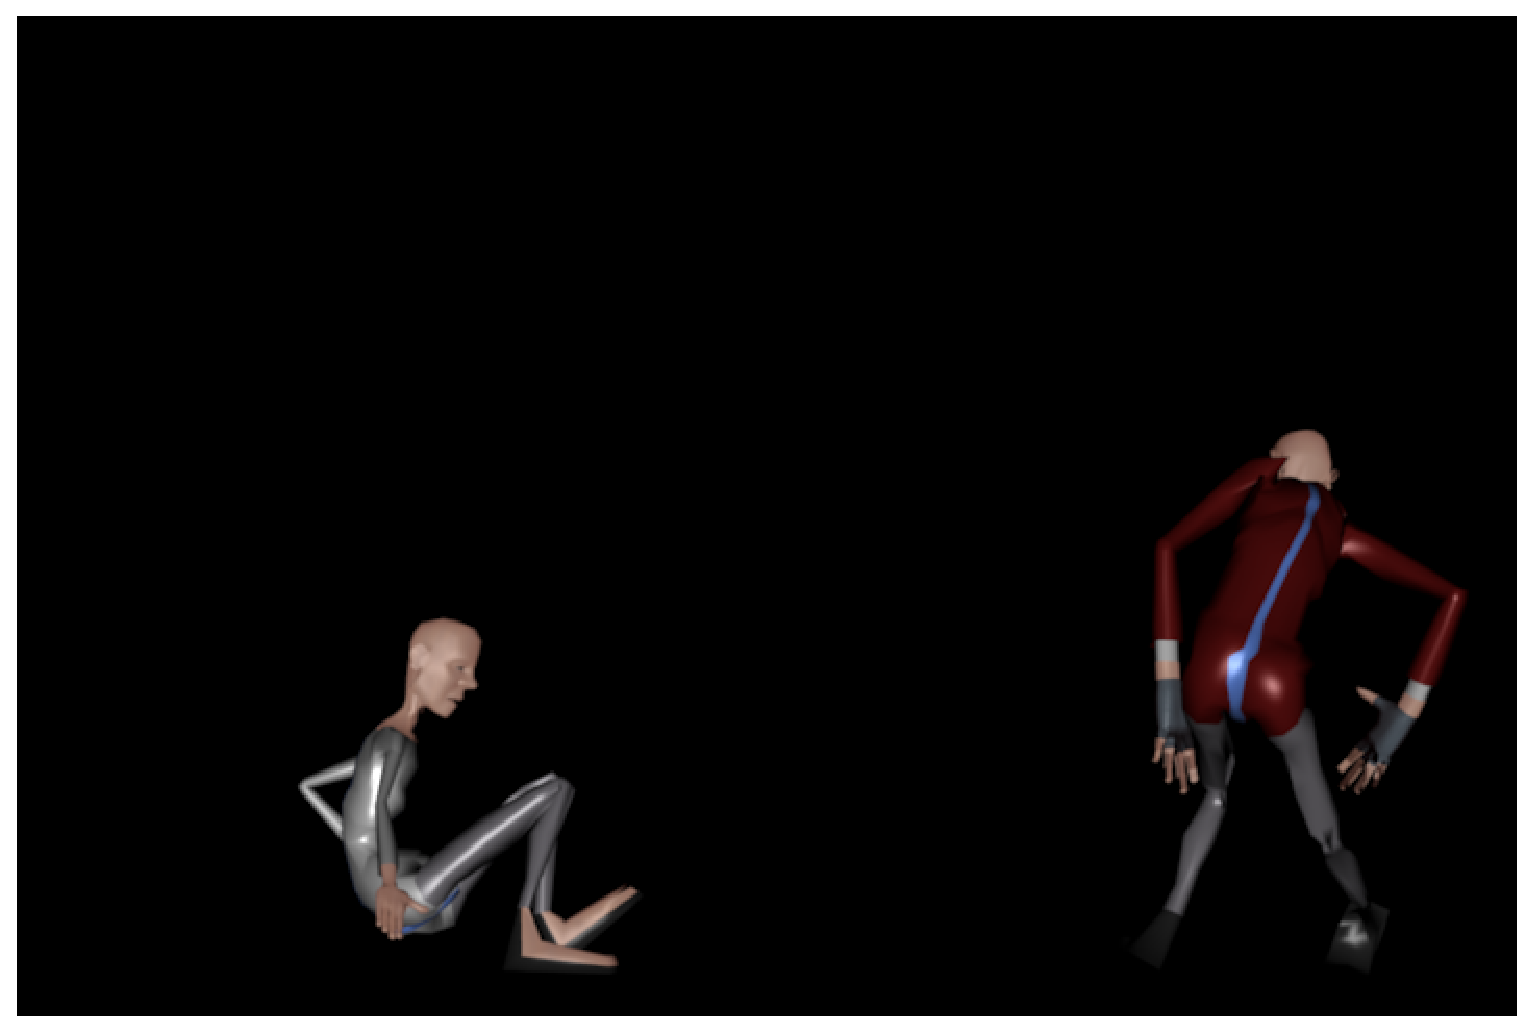
\psfig{file=compression/blender-foreground2-frame5.eps,width=1.9in}
\vspace{2pt}
\end{minipage}
\begin{minipage}{0.3\textwidth}
\centering
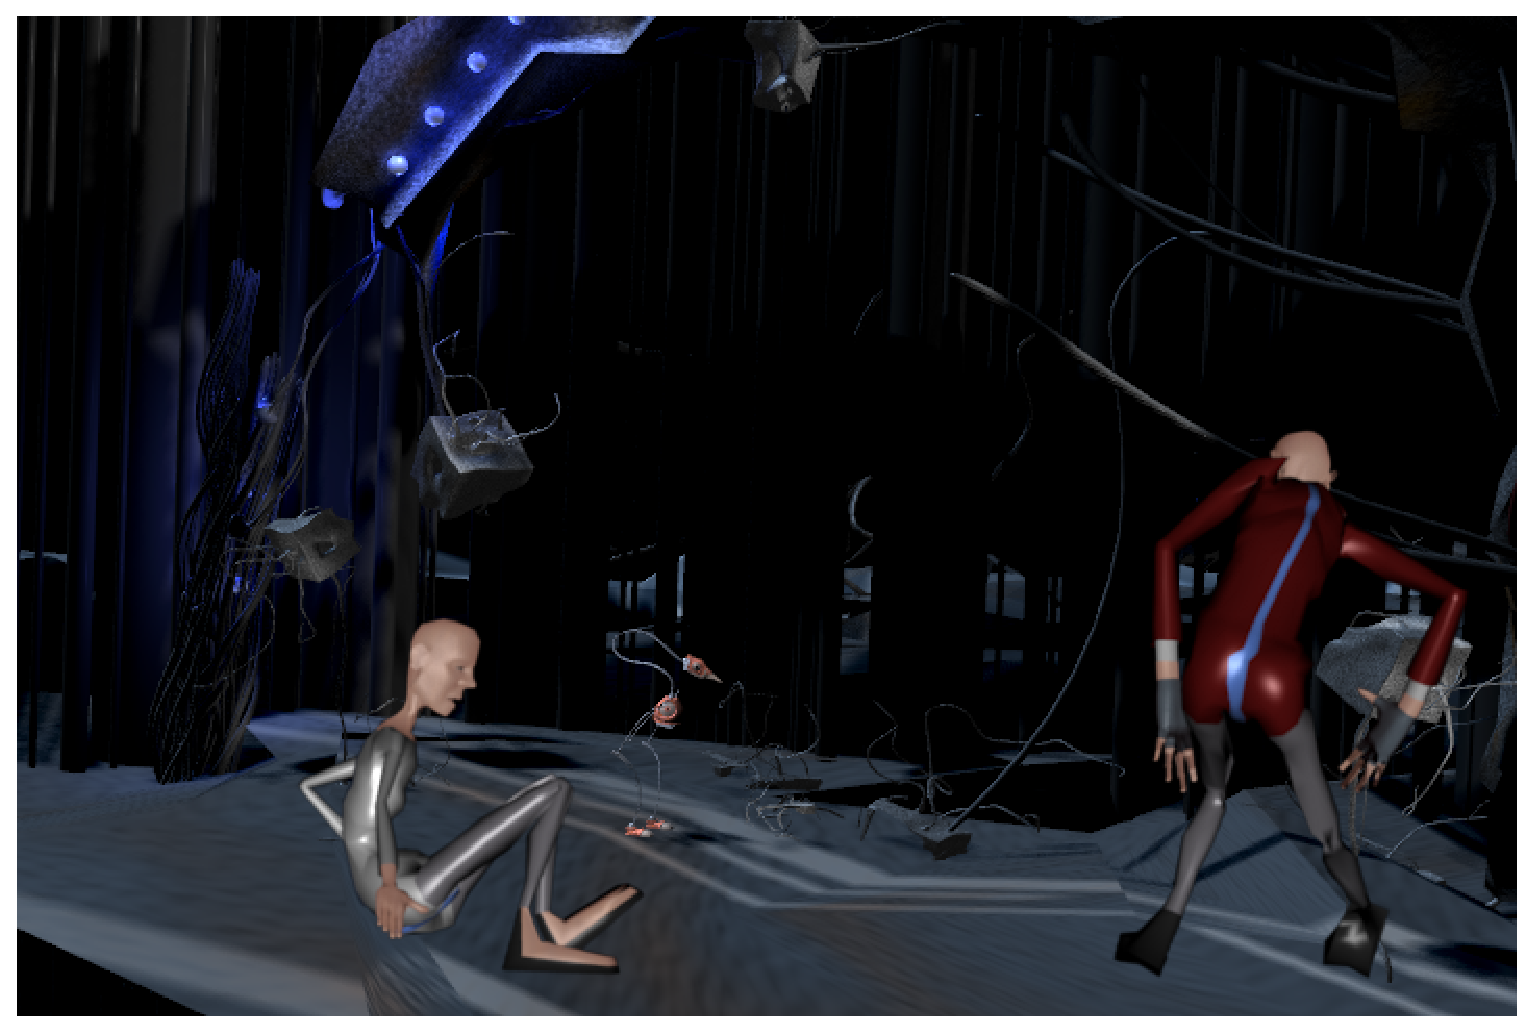
\psfig{file=compression/blender-composite-frame5.eps,width=1.9in}
\vspace{2pt}
\end{minipage}

{\small ~~~~~~~~~~~anim-scene1~~~~~~~~~~~~~~+~~~~~~~~~~~~~anim-character2~~~~~~~~~~~=~~~~~~~~~~~~~video composite~~~~~~~}

\begin{center}
\vspace{-3pt}
(a) Computer animation composite (alpha-under)
\end{center} \vspace{12pt}

\begin{minipage}{0.3\textwidth}
\centering

\psfig{file=compression/digvid-background1.eps,width=1.9in}
\vspace{2pt}
\end{minipage}
\begin{minipage}{0.3\textwidth}
\centering
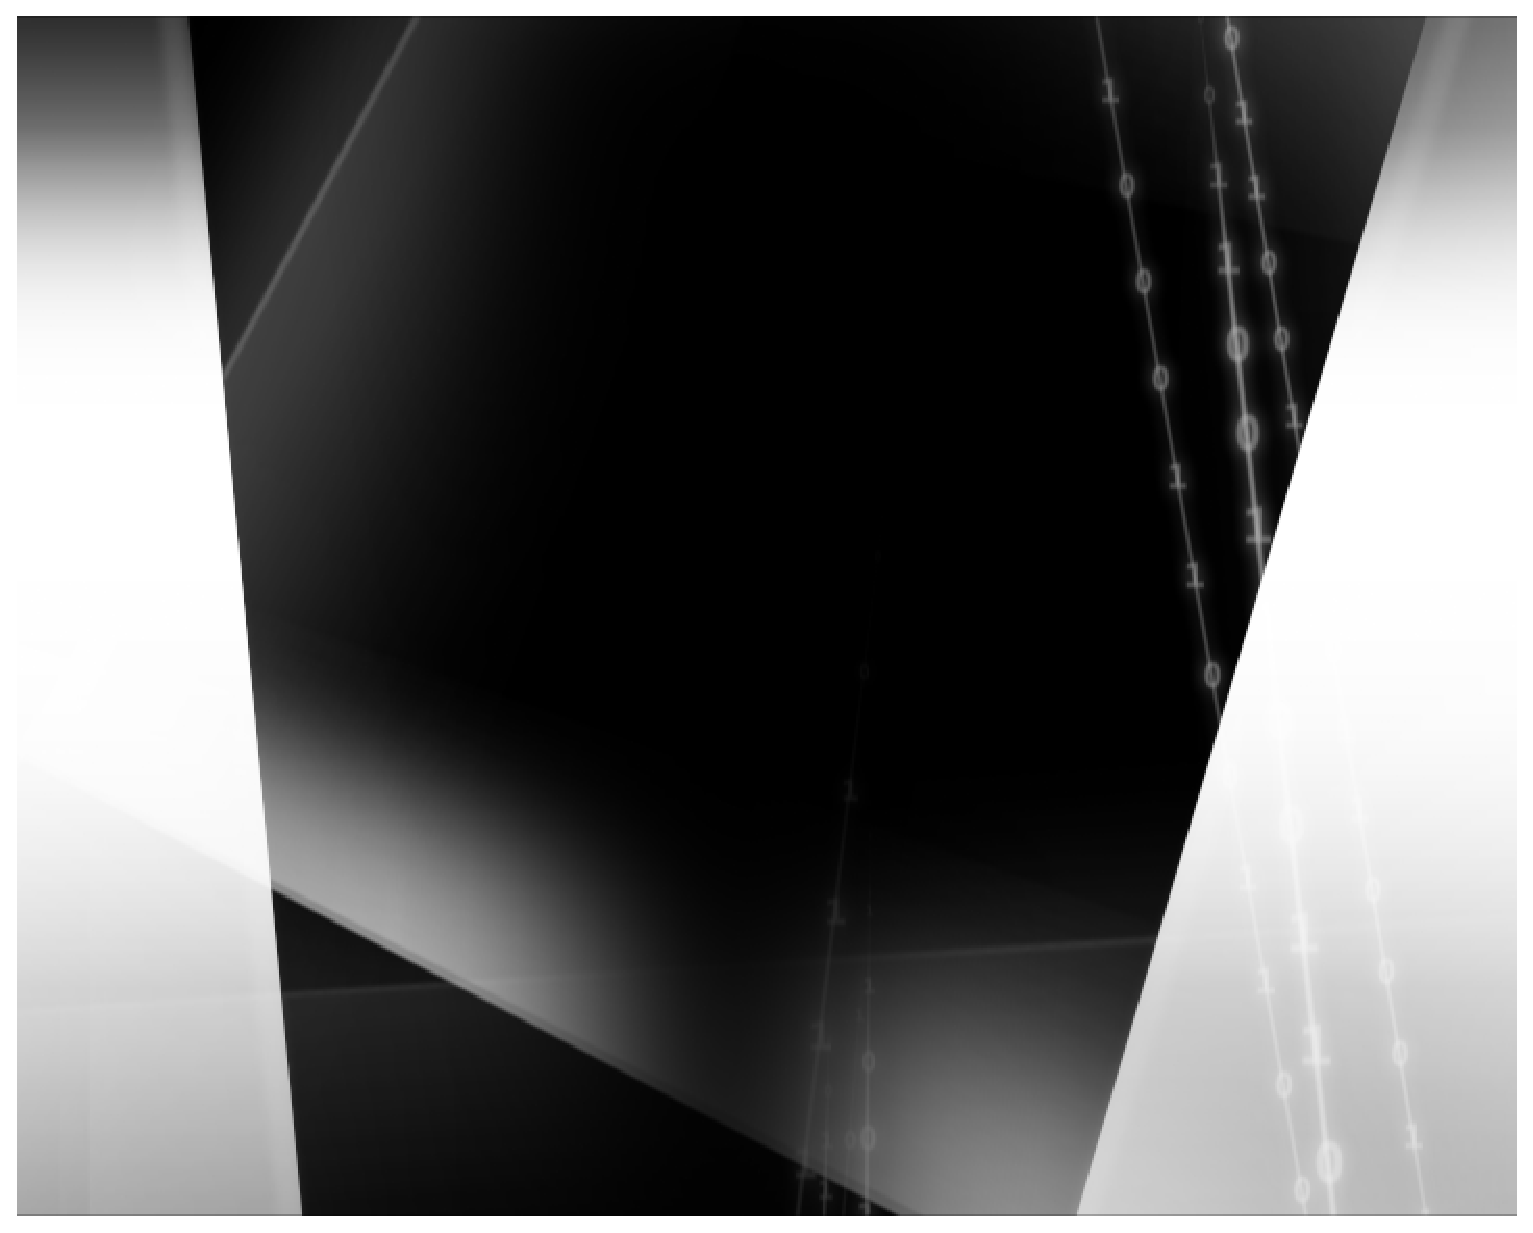
\psfig{file=compression/digvid-matte1-frame.eps,width=1.9in}
\vspace{2pt}
\end{minipage}
\begin{minipage}{0.3\textwidth}
\centering

\psfig{file=compression/digvid-composite.eps,width=1.9in}
\vspace{2pt}
\end{minipage}

{\small ~~~digvid-background1~~~~~~~~~~+~~~~~~~~~~~~digvid-matte-frame~~~~~~~~=~~~~~~~~~~~~~video composite~~~~~~~}

\begin{center}
\vspace{-3pt}
(b) Digital television composite (multiply)
\end{center}
\vspace{-3pt}
\caption{Examples of video compositing operations.\protect\label{fig:videos}}
\end{figure}

\begin{table*}[t]
\centering
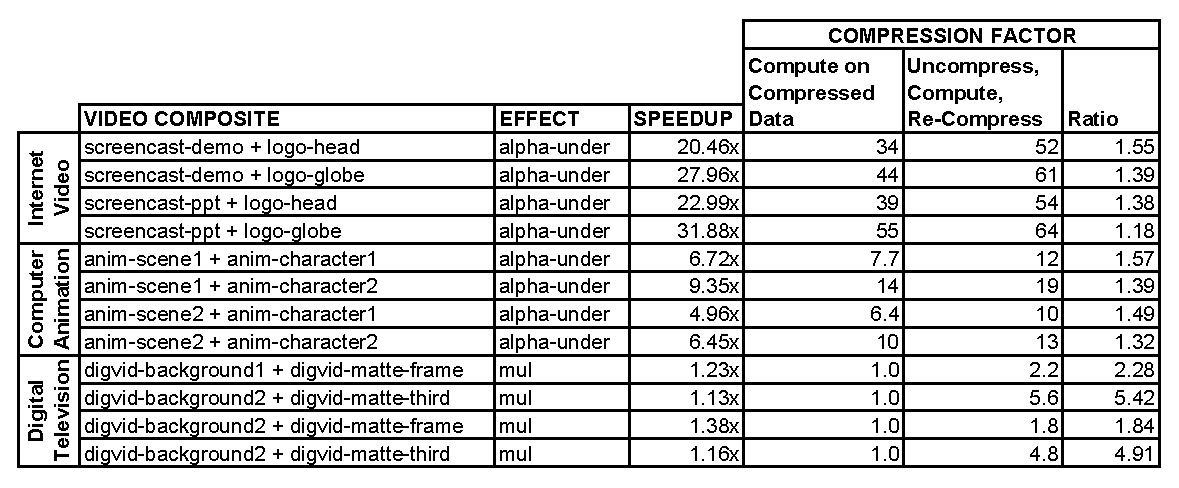
\psfig{file=compression/table-composite-speedup.eps,width=5.8in}
\caption[Table of results for composite transformations]{Results for composite transformations.
\protect\label{tab:composite-speedup}}
\end{table*}

Our optimized configuration operates in the compressed domain.
Outside of the auto-generated plugin, we patched three frame-copy
operations in
% actually four frame-copy operations, though one of them is a no-op
the Blender source code to copy only the compressed frame data rather
than the full frame dimensions.

\paragraph*{Results} Full results for the compositing operations appear in
Table~\ref{tab:composite-speedup}.  Figure~\ref{fig:composite-speedup}
illustrates the speedups, which range from 1.1x to 32x.  As in the
case of the pixel transformations, the speedups are closely correlated
with the compression factor of the resulting videos, a relationship
depicted in Figure~\ref{fig:speedup-scatter}.  The highly-compressed
screencasts enjoy the largest speedups (20x-32x), the computer
animations have intermediate speedups (5x-9x), while the digital
television content has negligible speedups (1.1x-1.4x).  Overall, the
speedups on video compositing (median = 6.6x) are lower than the pixel
transformations (median = 17x); this is because the compression
achieved on composite videos is roughly proportional to the minimum
compression across the two input files.

\begin{figure}[t]
\centering
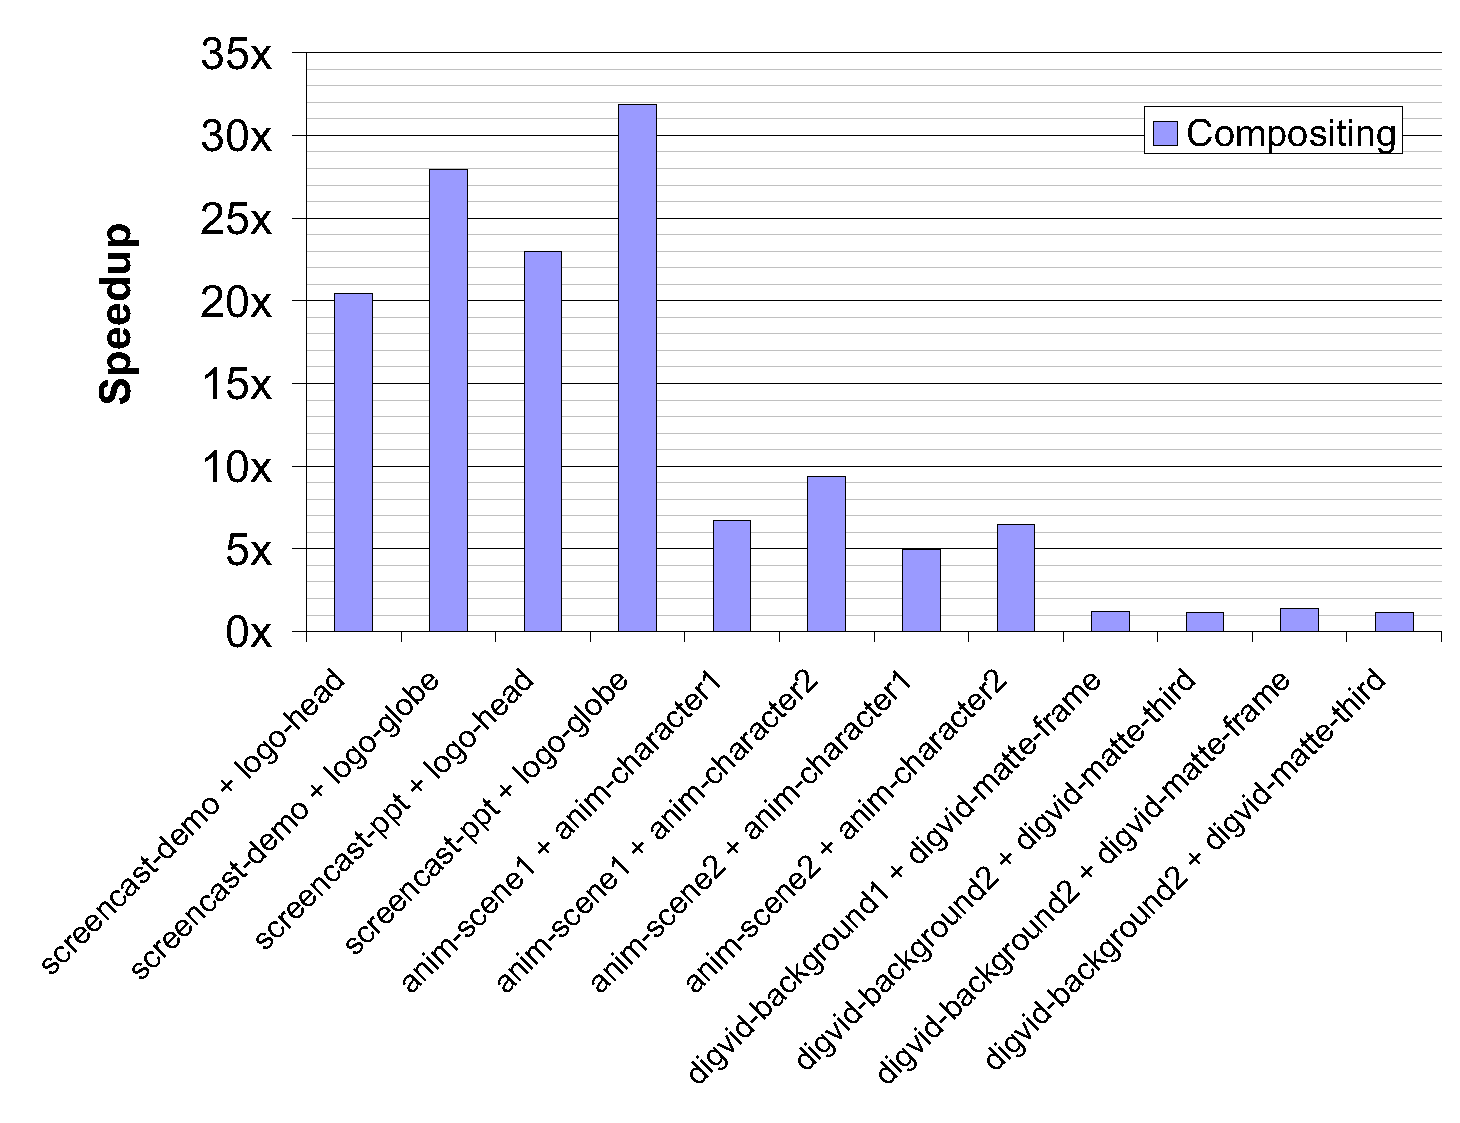
\psfig{file=compression/graph-speedup-composite.eps,width=4.355in}
\caption[Speedup graph for composite transformations]{Speedup on composite transformations.
\protect\label{fig:composite-speedup}}
\end{figure}

As for the pixel transformations, the composite videos produced by the
compressed processing technique would sometimes benefit from an
additional re-compression stage.  The last three columns in
Table~\ref{tab:composite-speedup} quantify this benefit by comparing
the compression factors achieved by compressed processing and normal
processing (including a re-compression step).  For screencasts and
computer animations, compressed processing preserves a sizable
compression factor (7.7x-44x), though the full re-compression can
further reduce file sizes by 1.2x to 1.6x.  For digital television,
the matting operations introduce a large amount of redundancy (black
regions), thereby enabling the re-compression stage to shrink the file
by 1.8x to 5.4x over the compressed processing technique.

Even if the composite transformation does not introduce any new
redundancy in the video, the compressed processing technique may
increase file sizes by ignoring a specific kind of redundancy in the
inputs.  Suppose that in the first frame, both inputs are 100\% black,
while in the second frame, one input is 100\% black and the other is
100\% white.  If the inputs are averaged, the second frame of output
will be 100\% gray and can be run-length encoded within the frame.
However, because the inputs have different kinds of redundancy on the
second frame (one is inter-frame, the other is intra-frame), the
technique is unable to detect the intra-frame redundancy in the output
and will instead produce N distinct pixels (all of them gray).  We
believe that this effect is small in practice, though we have yet to
quantify its impact in relation to the new redundancy introduced by a
transformation.  Future work will explore alternate data structures
for the compressed processing technique that may be able to preserve
this redundancy with low overhead.

\section{Related Work}
\label{sec:related}

Several other researchers have pursued the idea of operating directly
on compressed data formats.  The novelty of our work is two-fold:
first, in its focus on lossless compression formats, and second, in
its ability to map a flexible stream program, rather than a single
predefined operation, into the compressed domain.

Most of the previous work on mapping algorithms into the compressed
domain has focused on formats such as JPEG that utilize a Discrete
Cosine Transform (DCT) to achieve spatial
compression~\cite{smith98,dorai00,dugad01,feng03,mukherjee02,nang00,shen96,shen96b,shen98,smith96b,vasudev98}.
This task requires a different analysis, with particular attention
given to details such as the blocked decomposition of the image,
quantization of DCT coefficients, zig-zag ordering, and so-on.
Because there is also a run-length encoding stage in JPEG, our current
technique might find some application there; however, it appears that
techniques designed for JPEG have limited application to formats such
as LZ77.  
%Also, we are unaware of any previous methodology for
%translating a generic program to operate on compressed data; previous
%efforts have mapped each algorithm in a manual and ad-hoc way.

There has been some interest in performing compressed processing on
lossless encodings of black-and-white images.  Shoji presents the pxy
format for performing transpose and other affine
operations~\cite{shoji95}; the memory behavior of the technique was
later improved by Misra et al.~\cite{misra99}.  
%As described in
%Section~\ref{sec:formats}, the 
The pxy format lists the $(x,y)$ coordinate pairs at which a
black-and-white image changes color during a horizontal scan.  As
illustrated in Figure~\ref{fig:sj-example}, our technique can also
preserve a certain amount of compression during a transpose, though we
may achieve lesser compression than the pxy format due to our
one-dimensional view of the data.

Researchers have also considered the problem of pattern matching on
compressed text.  A randomized algorithm has been developed for
LZ77~\cite{farach98matching} while deterministic strategies exist for
LZ78 and LZW~\cite{navarro03regular,navarro05lzgrep}.  These solutions
are specialized to searching text; they do not apply to our
transformations, and our technique does not apply to theirs.

In the realm of programming languages, Swartz and Smith present RIVL,
a Resolution Independent Video Language~\cite{swartz95}.  The language
is used to describe a sequence of image transformations; this allows
the compiler to analyze the sequence and, via lazy evaluation, to
eliminate any operations that do not effect the final output.  Such a
technique is complementary to ours and could also be implemented using
StreamIt as the source language.

\section{Future Work}
\label{sec:future}

%% First, as the current transformation has the potential to increase the
%% size of the file, we plan to explore lightweight techniques for
%% re-compressing a data stream that is already partially compressed.
%% This should be straightforward in the case of Apple Animation; for
%% example, a run-length encoded unit can be extended without needing to
%% be rediscovered.

There remain rich areas for future work in computing on compressed
data.  First, the compressed processing technique can be applied far
beyond the current focus.  In its current form, the technique could be
evaluated on video operations such as thresholding, color depth
reduction, sepia toning, saturation adjustment, and color replacement.
With minor extensions, the technique can support video operations such
as cropping, padding, histograms, image flipping, sharpening, and
blurring.  The technique may also have applications in an embedded
setting, where it could offer power savings---for example, in
processing the RAW data format within digital cameras.  It may even be
possible to do sparse matrix operations using the technique; in
addition to compressing the locations of the zero elements, LZ77 would
also compress repetitive patterns in the non-zero elements.

Research is also underway to apply a similar technique to lossy,
DCT-based compression formats.  Because these formats represent a
linear encoding, they are subject to the linear optimizations
described in the previous chapter.  That is, a JPEG transcoder
typically performs an iDCT (during decompression), followed by the
user's transformation, followed by a DCT (during compression).  If the
user's transformation is also linear (e.g., color inversion) then all
three stages can be automatically collapsed, thereby eliminating the
decompression and re-compression steps.  Preliminary experiments in
this direction indicate speedups upwards of 10x.  Additional research
will be needed to support piecewise linear transformations, such as
brightness adjustment with saturation at the maximum brightness level.
By extending the framework to multiple compression formats, users will
be able to write their transformations once, in a high-level language,
and rely on the compiler to map the computations to each of the
compressed domains.

While we formulated our transformation in terms of a streaming model,
the techniques can be applied within other functional and
general-purpose languages so long as the right information is
available and certain constraints are satisfied.  The transformation
relies on a regular pattern of data access; we use a streaming
abstraction, but structured iteration over arrays could also suffice.
We rely on static data rates in actors, which could also be expressed
as functions with a fixed number of arguments and return values.
Actors (functions) must be pure, without side effects or unresolvable
dependences on potentially mutable data.  While these properties are
intrinsic to a language such as StreamIt, they also come naturally in
most functional languages and may be adaptable to general-purpose
languages in the form of a runtime library with a restricted API.

\section{Chapter Summary}

%% Many of the applications that will drive the next generation of
%% computing systems---digital video editing, computer vision, computer
%% graphics and animation---operate on image and video formats that are
%% universally stored in compressed data formats.  

In order to accelerate operations on compressible data, this chapter
presents a general technique for translating stream programs into the
compressed domain.  Given a natural program that operates on
uncompressed data, our transformation outputs a program that directly
operates on the compressed data format.  We support lossless
compression formats based on LZ77.  In the general case, the
transformed program may need to partially decompress the data to
perform the computation, though this decompression is minimized
throughout the process and significant compression ratios are
preserved without resorting to an explicit re-compression step.

We implemented some of our transformations in the StreamIt compiler
and demonstrated excellent speedups.  Across a suite of 12 videos in
Apple Animation format, computing directly on compressed data offers a
speedup roughly proportional to the compression ratio.  For pixel
transformations (brightness, contrast, inverse) speedups range from
2.5x to 471x, with a median of 17x; for video compositing operations
(overlays and mattes) speedups range from 1.1x to 32x, with a median
of 6.6x.  While previous researchers have used special-purpose
compressed processing techniques to obtain speedups on lossy,
DCT-based codecs, we are unaware of a comparable demonstration for
lossless video compression.  As digital films and animated features
have embraced lossless formats for the editing process, the speedups
obtained may have practical value.
